% !TeX program = xelatex
% !TeX encoding = UTF-8
% Presentazione revisionata: Isocrona · Datazione radiometrica
% Basata sul materiale originale fornito dall'autore e sul template M01_Pensare_con_i_dati.tex
% Compilazione: xelatex -interaction=nonstopmode M19_Isocrona.tex (due passaggi)
% Diagrammi TikZ e figure statistiche vettoriali; sorgenti R e dati inclusi.
% 32 slide. Materiali del corso e impaginazione della serie planetaria.
\RequirePackage{fix-cm}
\documentclass[12pt,aspectratio=1610]{beamer}
\geometry{paperwidth=20cm,paperheight=12.5cm}
\usepackage[italian,provide=*]{babel}
\usepackage{fontspec,adjustbox,tabularx}
\IfFontExistsTF{NimbusSans-Regular.otf}{
\setsansfont{NimbusSans-Regular.otf}[BoldFont=NimbusSans-Bold.otf,ItalicFont=NimbusSans-Italic.otf,BoldItalicFont=NimbusSans-BoldItalic.otf]
\setmainfont{NimbusSans-Regular.otf}[BoldFont=NimbusSans-Bold.otf,ItalicFont=NimbusSans-Italic.otf,BoldItalicFont=NimbusSans-BoldItalic.otf]
}{
\setsansfont{TeX Gyre Heros}
\setmainfont{TeX Gyre Heros}
}
\IfFontExistsTF{DejaVu Sans Mono}{
\setmonofont{DejaVu Sans Mono}[Scale=.88]
}{\setmonofont{Latin Modern Mono}[Scale=.88]}
\usefonttheme{professionalfonts}
\usepackage{amsmath,amssymb,booktabs,array,graphicx,tikz,bookmark}
\usetikzlibrary{calc,positioning,arrows.meta}
\graphicspath{{Figure/}}
\definecolor{Paper}{HTML}{F8F6F1}
\definecolor{Ink}{HTML}{253344}
\definecolor{Navy}{HTML}{15283E}
\definecolor{Quantum}{HTML}{5146A5}
\definecolor{Classical}{HTML}{087C74}
\definecolor{Muted}{HTML}{657180}
\definecolor{Rule}{HTML}{D6DAD9}
\definecolor{Night}{HTML}{112236}
\definecolor{Lilac}{HTML}{ABB5FF}
\definecolor{Mint}{HTML}{72D8C8}
\setbeamercolor{background canvas}{bg=Paper}
\setbeamercolor{normal text}{fg=Ink}
\setbeamertemplate{navigation symbols}{}
\setbeamertemplate{headline}{}
\setbeamertemplate{footline}{}
\setbeamersize{text margin left=0pt,text margin right=0pt}
\hypersetup{colorlinks=true,linkcolor=Classical,urlcolor=Classical,pdfpagemode=UseOutlines,pdfstartview=Fit,
 pdftitle={Isocrona · Datazione radiometrica},pdfauthor={GeoStat Lab · materiali di Marzio De Corato},
 pdfsubject={GeoStat Lab · M19}}
\bookmarksetup{open,openlevel=0,depth=2}
\newsavebox{\BodyBox}
\newsavebox{\SideBox}
\newsavebox{\RecallBox}
\newsavebox{\TitleBox}
\newcommand{\MeasureBox}[2]{\typeout{REVIEWBOX:#1:\the\wd#2:\the\ht#2:\the\dp#2}}

% Revisione completa: diagrammi TikZ, formalismo e box R.
\usepackage[most]{tcolorbox}
\usepackage{listings}
\usetikzlibrary{fit,backgrounds,matrix,decorations.pathreplacing}
\definecolor{GeoA}{HTML}{1D7890}
\definecolor{GeoB}{HTML}{C57E42}
\definecolor{GeoC}{HTML}{7363AA}
\definecolor{GeoTint}{HTML}{F0F4F3}
\lstdefinestyle{GeoR}{language=R,basicstyle=\ttfamily\fontsize{9.2}{12.2}\selectfont,
 keywordstyle=\color{Quantum}\bfseries,commentstyle=\color{Classical},stringstyle=\color{GeoB},
 numbers=left,numberstyle=\tiny\color{Muted},numbersep=4pt,showstringspaces=false,
 columns=fullflexible,keepspaces=true,breaklines=true,xleftmargin=1.15em,
 frame=none,aboveskip=0pt,belowskip=0pt,tabsize=2}
\newsavebox{\PilotLeftBox}
\newsavebox{\PilotRightBox}
\newcommand{\PLabel}[1]{\par{\color{Classical}\bfseries\fontsize{9}{11}\selectfont\MakeUppercase{#1}}\par\vspace{1.8mm}}
\newcommand{\PBody}[1]{\par{\fontsize{11.3}{14.8}\selectfont #1\par}}
\newcommand{\PSmall}[1]{\par{\fontsize{9.8}{13.1}\selectfont #1\par}}
\newcommand{\PCode}[2]{%
\begin{tcolorbox}[enhanced,arc=1.8mm,boxrule=.65pt,
  colback=white,colframe=Classical!75!Navy,colbacktitle=Navy,
  coltitle=white,fonttitle=\bfseries\fontsize{9.6}{12}\selectfont,
  title={#1},left=1.7mm,right=1.3mm,top=1.5mm,bottom=1.3mm,
  before skip=1mm,after skip=1mm]
\lstinputlisting[style=GeoR]{Codice/#2}
\end{tcolorbox}}
\newcommand{\PInfo}[1]{%
\begin{tcolorbox}[enhanced,arc=1.6mm,boxrule=.55pt,colback=GeoTint,
 colframe=Rule!80!Classical,left=2.3mm,right=2.3mm,top=2mm,bottom=2mm,
 before skip=1mm,after skip=1mm]
\PSmall{#1}\end{tcolorbox}}
\tikzset{
 pFlow/.style={draw=Classical!45,fill=white,rounded corners=2mm,
  line width=.7pt,align=center,minimum height=1.1cm,font=\sffamily\fontsize{10}{12}\selectfont},
 pEdge/.style={-{Latex[length=2.3mm]},draw=Classical,line width=.95pt},
 pGroup/.style={draw=Rule,fill=white,rounded corners=2mm,line width=.65pt},
 pDotA/.style={circle,fill=GeoA,inner sep=1.25pt},
 pDotB/.style={circle,fill=GeoB,inner sep=1.25pt},
 pDotC/.style={circle,fill=GeoC,inner sep=1.25pt}
}
\newcommand{\PilotChrome}[4]{%
  \node[anchor=north west,inner sep=0,text width=17.7cm] at ([xshift=.95cm,yshift=-.55cm]current page.north west) {\color{Navy}\bfseries\fontsize{20.6}{24.5}\selectfont #1};
  \node[anchor=north east,inner sep=0] at ([xshift=19.05cm,yshift=-.14cm]current page.north west) {\color{Classical}\fontsize{8}{10}\selectfont\hyperlink{slide2}{#2}};
  \draw[Classical,line width=1.2pt] ([xshift=.95cm,yshift=-1.7cm]current page.north west)--([xshift=2.35cm,yshift=-1.7cm]current page.north west);
  \draw[Rule,line width=.65pt] ([xshift=.95cm,yshift=-10.36cm]current page.north west)--([xshift=19.05cm,yshift=-10.36cm]current page.north west);
  \node[anchor=north west,inner sep=0] at ([xshift=.96cm,yshift=-10.55cm]current page.north west) {\color{Classical}\bfseries\fontsize{9.1}{12}\selectfont DA RICORDARE};
  \node[anchor=north west,inner sep=0,text width=14.3cm] at ([xshift=4.2cm,yshift=-10.53cm]current page.north west) {\color{Ink}\fontsize{10.3}{13.8}\selectfont #4};
  \draw[Rule,line width=.35pt] ([xshift=.95cm,yshift=-11.92cm]current page.north west)--([xshift=19.05cm,yshift=-11.92cm]current page.north west);
  \node[anchor=north west,inner sep=0] at ([xshift=.95cm,yshift=-12.06cm]current page.north west) {\color{Muted}\fontsize{7.7}{9.2}\selectfont Isocrona · Datazione radiometrica};
  \node[anchor=north east,inner sep=0] at ([xshift=19.05cm,yshift=-12.06cm]current page.north west) {\color{Muted}\fontsize{7.7}{9.2}\selectfont #3/32};
}


% Stili comuni per i diagrammi scientifici della revisione completa.
\tikzset{
 pAxis/.style={-{Latex[length=2mm]},draw=Muted,line width=.65pt},
 pNote/.style={font=\sffamily\fontsize{9}{11.5}\selectfont,text=Muted,align=center},
 pLabel/.style={font=\sffamily\fontsize{10}{12.5}\selectfont,text=Ink,align=center}
}
\newsavebox{\FullWideBox}
\setlength{\emergencystretch}{1em}




\newcommand{\PLab}[2]{\par{\color{Classical}\bfseries\fontsize{9}{11}\selectfont
\href{#1}{\MakeUppercase{#2}}}\par\vspace{1.8mm}}

\definecolor{Measure}{HTML}{A05B10}\definecolor{Rose}{HTML}{9B4564}\definecolor{Wash}{HTML}{EAE7F6}\definecolor{Gold}{HTML}{EEC184}
\tikzset{arr/.style={-{Stealth[length=2mm]},line width=.8pt,draw=Classical}}
\newcommand{\Colonna}[2]{\begin{adjustbox}{max totalsize={#1}{7.95cm},valign=t}\begin{minipage}[t]{#1}\raggedright\fontsize{11.3}{14.8}\selectfont #2\end{minipage}\end{adjustbox}}
\begin{document}

\begin{frame}[plain]\hypertarget{slide1}{}\bookmark[level=0,page=1]{Isocrona}
\begin{tikzpicture}[remember picture,overlay]
\fill[Night](current page.south west) rectangle(current page.north east);
\IfFileExists{Scena/copertina.jpg}{\node[inner sep=0] at(current page.center){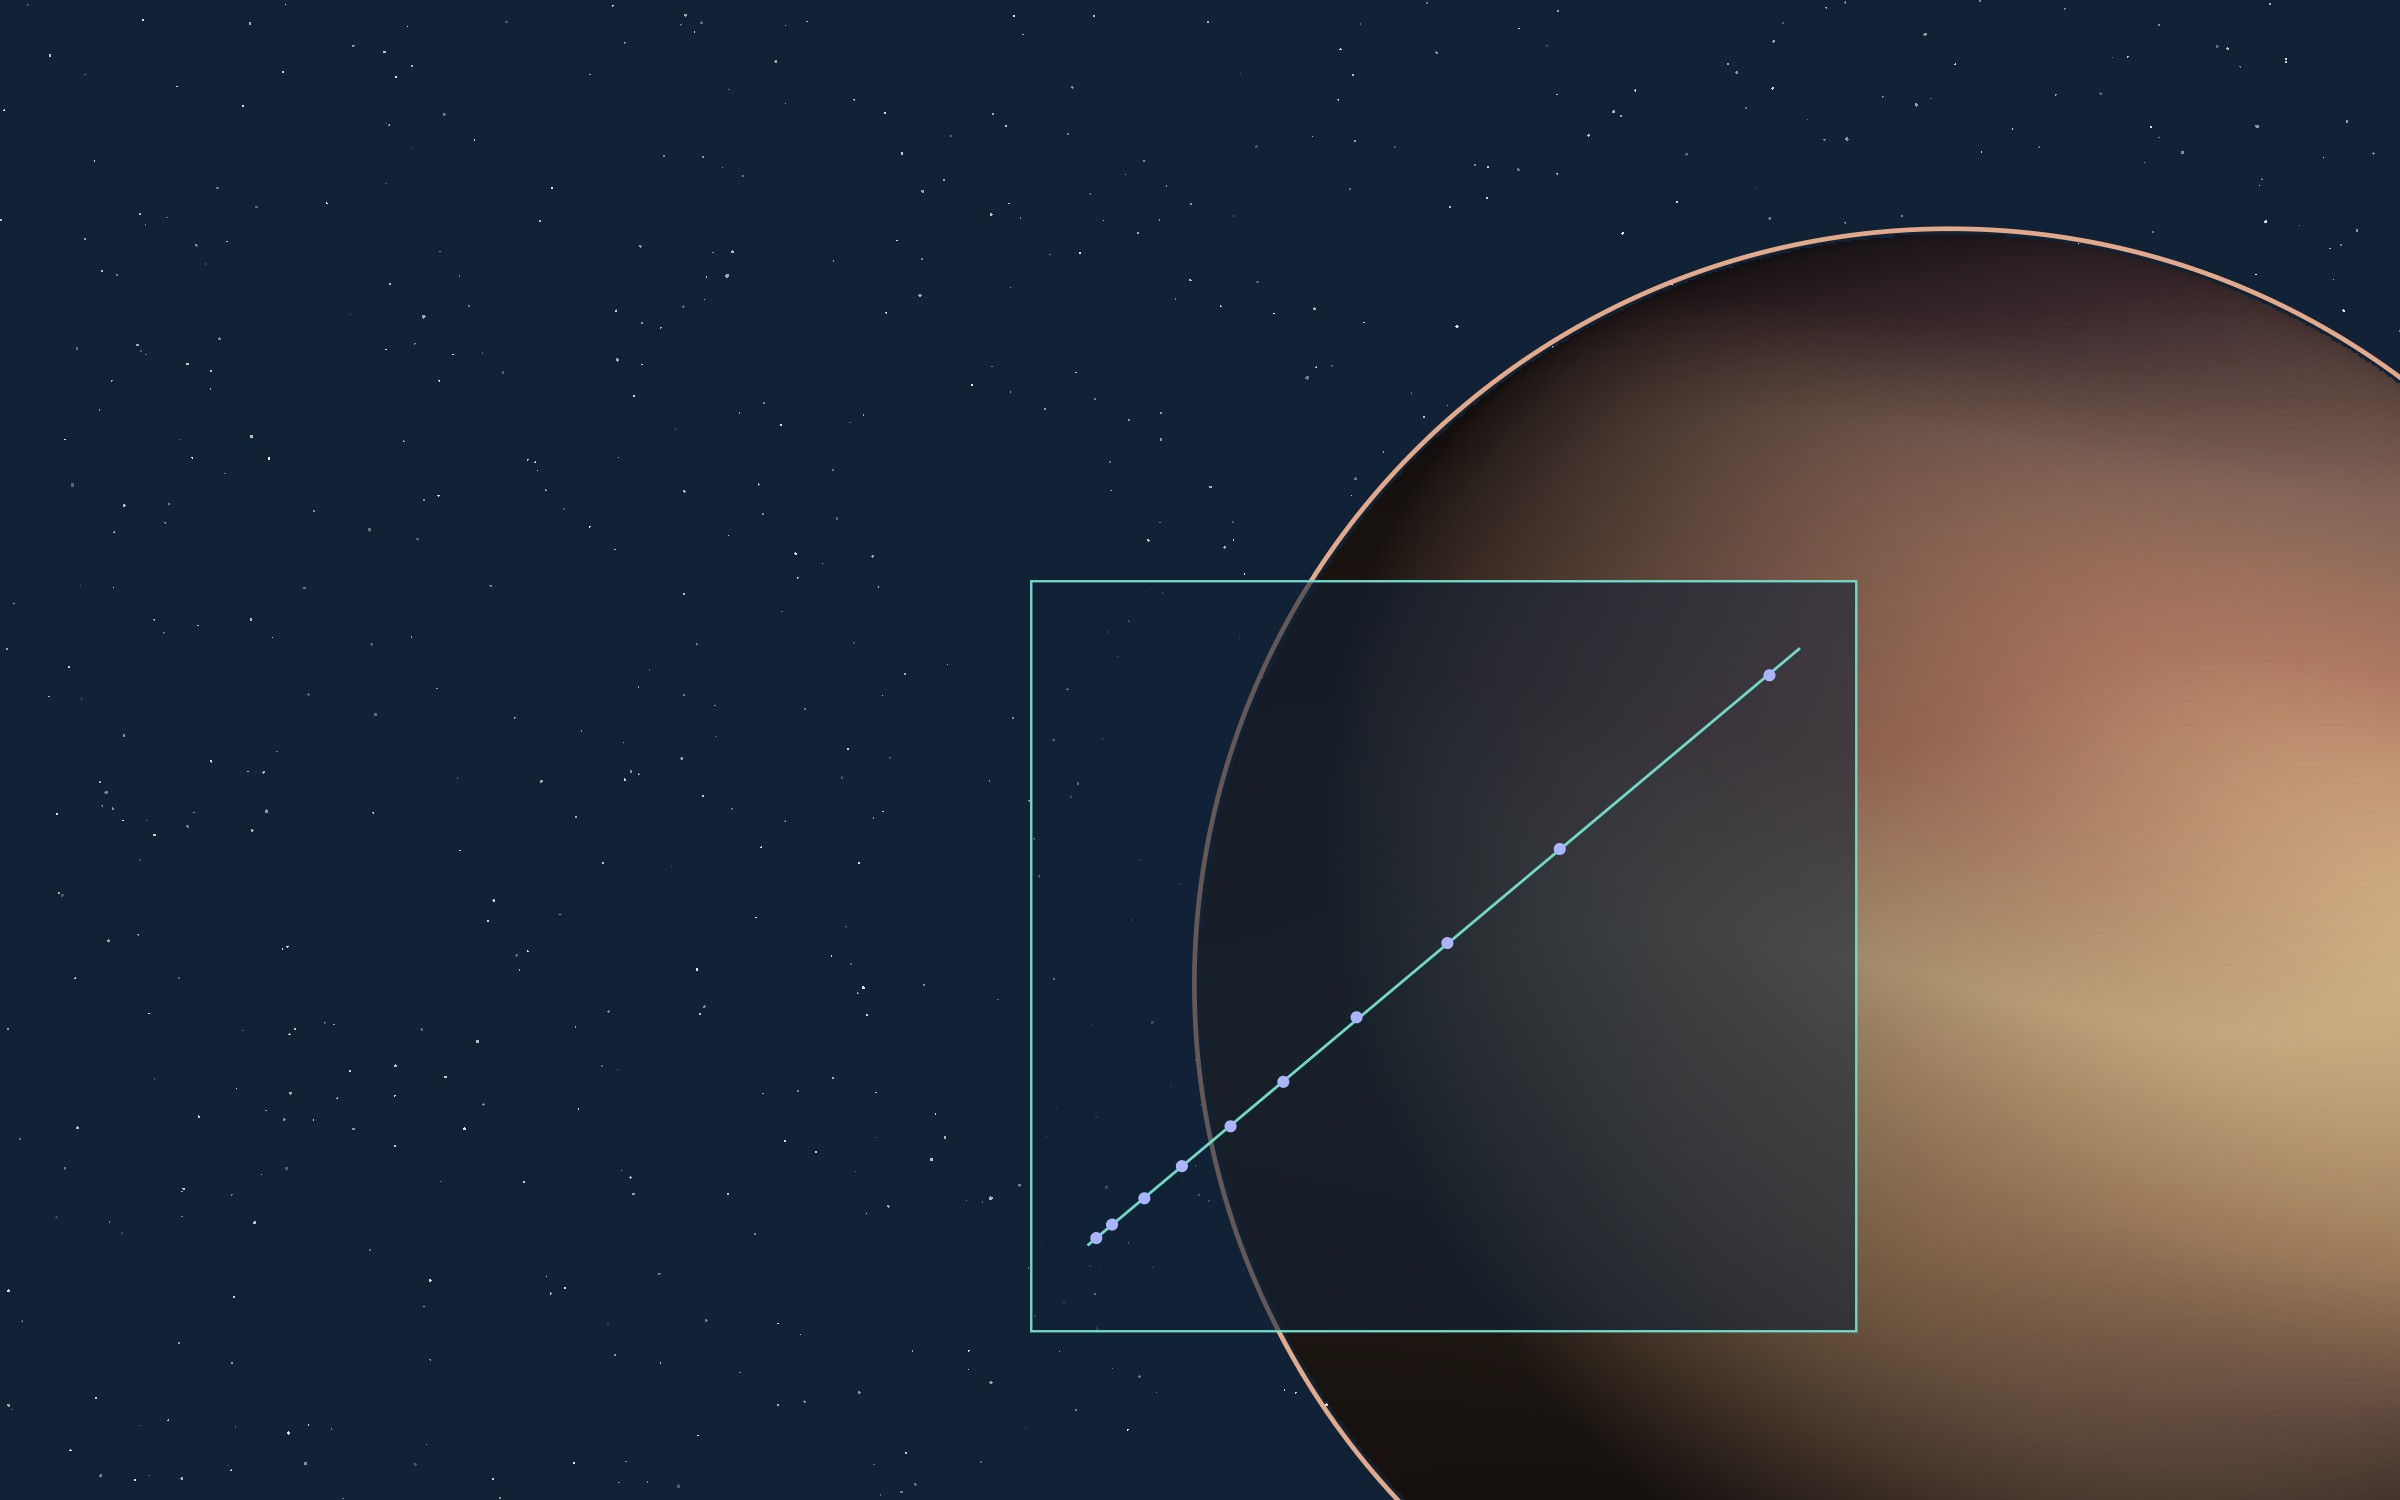
\includegraphics[width=20cm,height=12.5cm]{Scena/copertina.jpg}};}{}
\node[anchor=north west,inner sep=0] at([xshift=1.05cm,yshift=-1.10cm]current page.north west){\color{Mint}\bfseries\fontsize{23}{28}\selectfont ISOCRONA};
\node[anchor=north west,inner sep=0] at([xshift=1.07cm,yshift=-2.16cm]current page.north west){\color{white}\fontsize{9}{12}\selectfont MODULO M19 · SCIENZE DELLA TERRA};
\draw[Mint,line width=1.5pt]([xshift=1.07cm,yshift=-2.78cm]current page.north west)--([xshift=2.6cm,yshift=-2.78cm]current page.north west);
\node[anchor=north west,inner sep=0] at([xshift=1.05cm,yshift=-3.35cm]current page.north west){\begin{minipage}{9.2cm}\raggedright\color{white}\bfseries\fontsize{28.5}{34.5}\selectfont Datazione\\radiometrica\end{minipage}};
\node[anchor=north west,inner sep=0] at([xshift=1.07cm,yshift=-7.88cm]current page.north west){\begin{minipage}{8.9cm}\raggedright\color{Lilac}\fontsize{12.2}{17}\selectfont Rapporti isotopici che diventano età\end{minipage}};
\node[anchor=north west,inner sep=0] at([xshift=1.07cm,yshift=-8.70cm]current page.north west){\begin{minipage}{8.9cm}\raggedright\color{white!75}\fontsize{10.3}{14.5}\selectfont Isocrone, regressione di York, MSWD e incertezza delle età\end{minipage}};
\node[anchor=north west,inner sep=0] at([xshift=1.07cm,yshift=-10.52cm]current page.north west){\color{white}\fontsize{10.5}{14}\selectfont GeoStat Lab · corso di Marzio De Corato};
\node[anchor=north west,inner sep=0] at([xshift=1.07cm,yshift=-11.17cm]current page.north west){\color{Mint}\fontsize{8.8}{11}\selectfont\href{https://creativecommons.org/licenses/by-nc-sa/4.0/}{Impaginazione da Tessera · CC BY-NC-SA 4.0}};
\end{tikzpicture}\end{frame}

\begin{frame}[plain]\hypertarget{slide2}{}
\bookmark[level=1,page=2]{Indice della presentazione}
\begin{tikzpicture}[remember picture,overlay]
\PilotChrome{Indice della presentazione}{PERCORSO}{2}{I titoli dell’indice aprono i capitoli. Il nome del capitolo in alto riporta a questa pagina.}
\node[anchor=north west,inner sep=0] at([xshift=.96cm,yshift=-2.12cm]current page.north west){\Colonna{9.40cm}{\PLabel{Capitoli}
{\fontsize{10.7}{13.5}\selectfont\hyperlink{slide4}{Il decadimento come orologio\hfill 4}\par}\vspace{.16cm}
{\fontsize{10.7}{13.5}\selectfont\hyperlink{slide10}{L’isocrona\hfill 10}\par}\vspace{.16cm}
{\fontsize{10.7}{13.5}\selectfont\hyperlink{slide17}{MSWD e dispersione in eccesso\hfill 17}\par}\vspace{.16cm}
{\fontsize{10.7}{13.5}\selectfont\hyperlink{slide24}{Incertezza e confronto delle età\hfill 24}\par}\vspace{.16cm}
}};
\node[anchor=north west,inner sep=0] at([xshift=10.85cm,yshift=-2.12cm]current page.north west){\Colonna{8.16cm}{\PLabel{Percorso di lettura}
\PBody{Dieci campioni di un granito e otto di un filone riportano i rapporti isotopici del sistema Rb-Sr con le loro incertezze; quindici zirconi dello stesso granito hanno una data U-Pb. Il percorso va dalla legge del decadimento all’isocrona, alla regressione con errori su entrambi gli assi, alla MSWD e al confronto fra età.}
\PInfo{Le pagine Scenario A e Confronto riprendono gli esperimenti nel browser. I valori di partenza del simulatore possono differire dal caso guida.}
\href{https://marzione00.github.io/Lab_Geo/\#modulo-M19}{\color{Classical}\bfseries Apri gli esperimenti di Isocrona}}};
\end{tikzpicture}\end{frame}

\begin{frame}[plain]\hypertarget{slide3}{}
\bookmark[level=1,page=3]{Quanti anni ha il granito, e con quale incertezza?}
\begin{tikzpicture}[remember picture,overlay]
\PilotChrome{Quanti anni ha il granito, e con quale incertezza?}{IL CASO GUIDA}{3}{Un’età radiometrica è una stima: va riportata con la sua incertezza e con il modello che la produce.}
\node[anchor=north west,inner sep=0] at([xshift=.96cm,yshift=-2.12cm]current page.north west){\Colonna{9.40cm}{{\centering\resizebox{.97\linewidth}{!}{\begin{tikzpicture}[x=1cm,y=1cm,every node/.append style={anchor=center,inner sep=.3333em}]
\foreach \x/\n/\t/\col in {0.9/1/Decadimento/GeoA,3.0/2/Isocrona/GeoC,5.1/3/MSWD/GeoA,7.2/4/Incertezza delle età/GeoB}{
 \draw[\col,fill=\col!8,rounded corners=4pt,line width=.8pt] (\x-.95,1.25) rectangle(\x+.95,3.35);
 \node[font=\bfseries\fontsize{15}{18}\selectfont,text=\col] at(\x,2.75){\n};
 \node[pNote,text width=1.75cm] at(\x,1.85){\t};}
\foreach \x in {1.85,3.95,6.05}{\draw[pEdge] (\x,2.3)--(\x+.2,2.3);}
\draw[Rule,line width=.6pt] (0,.75)--(8.15,.75);
\node[pNote] at(4.08,.35){Un rapporto isotopico diventa un’età con una retta e i suoi errori.};
\end{tikzpicture}
}\par}
}};
\node[anchor=north west,inner sep=0] at([xshift=10.85cm,yshift=-2.12cm]current page.north west){\Colonna{8.16cm}{\PLabel{Il caso}
\PBody{Dieci campioni sintetici di un granito e otto di un filone che lo attraversa riportano i rapporti ${}^{87}$Rb/${}^{86}$Sr e ${}^{87}$Sr/${}^{86}$Sr misurati, con le deviazioni standard analitiche. Quindici zirconi del granito hanno una data U-Pb ciascuno. I dati sono generati con età note, per confrontare le stime con i valori veri.}
\PInfo{Seguiremo i dati dalla legge del decadimento all’isocrona, alla regressione di York, alla MSWD e alla combinazione delle incertezze, fino al confronto fra l’età Rb-Sr e quella degli zirconi.}
}};
\end{tikzpicture}\end{frame}

\begin{frame}[plain]\hypertarget{slide4}{}
\bookmark[level=0,page=4]{Il decadimento come orologio}
\bookmark[level=1,page=4]{Quanto lentamente decade il rubidio?}
\begin{tikzpicture}[remember picture,overlay]
\PilotChrome{Quanto lentamente decade il rubidio?}{IL DECADIMENTO COME OROLOGIO}{4}{Il tempo di dimezzamento è $\log 2/\lambda$; un rapporto figlio/genitore si traduce in un’età.}
\node[anchor=north west,inner sep=0] at([xshift=.96cm,yshift=-2.12cm]current page.north west){\Colonna{9.40cm}{\PLabel{Domanda}
\PBody{La costante di decadimento di ${}^{87}$Rb raccomandata nel 2015 da IUPAC e IUGS è $1{,}3972\cdot10^{-11}$ per anno. Qual è il tempo di dimezzamento? Che età corrisponde a un rapporto fra ${}^{87}$Sr radiogenico e ${}^{87}$Rb di 0,0042?}
\vspace{.35cm}\PLabel{Interpretazione}
\PBody{Il tempo di dimezzamento è 49,61 miliardi di anni. Un rapporto di 0,0042 corrisponde a circa 300 milioni di anni: in questo intervallo decade lo 0,42\% del rubidio.}
}};
\node[anchor=north west,inner sep=0] at([xshift=10.85cm,yshift=-2.12cm]current page.north west){\Colonna{8.16cm}{\begin{tcolorbox}[enhanced,arc=1.7mm,boxrule=.6pt,colback=white,colframe=Classical!60!Navy,colbacktitle=Navy,coltitle=white,fonttitle=\bfseries\small,title={R · calcolo riproducibile},left=1.7mm,right=1.3mm,top=1.1mm,bottom=1.1mm,before skip=1mm,after skip=1.0mm]\lstinputlisting[style=GeoR,language=R]{Codice/capitolo-01.R}\end{tcolorbox}
\PLabel{Risultato in R}
\begin{tcolorbox}[colback=GeoTint,colframe=Rule,boxrule=.5pt,arc=1.4mm,left=2mm,right=1mm,top=1mm,bottom=1mm]{\fontsize{8.6}{11.4}\selectfont\ttfamily \mbox{dimezzamento\_Ga\ \ \ \ \ \ \ \ \ \ eta\_Ma}\\\mbox{\ \ \ \ \ \ \ \ \ \ 49.61\ \ \ \ \ \ \ \ \ \ 299.97}}\end{tcolorbox}}};
\end{tikzpicture}\end{frame}

\begin{frame}[plain]\hypertarget{slide5}{}
\bookmark[level=1,page=5]{Il genitore decade, il figlio si accumula}
\begin{tikzpicture}[remember picture,overlay]
\PilotChrome{Il genitore decade, il figlio si accumula}{IL DECADIMENTO COME OROLOGIO}{5}{In un sistema chiuso l’età dipende dal rapporto fra figlio radiogenico e genitore rimasto.}
\node[anchor=north west,inner sep=0] at([xshift=.96cm,yshift=-2.12cm]current page.north west){\Colonna{9.40cm}{{\centering\resizebox{0.94\linewidth}{!}{\begin{tikzpicture}[x=1cm,y=1cm,every node/.append style={anchor=center,inner sep=.3333em}]
\draw[-{Latex[length=2mm]},Ink,line width=.6pt] (0,0)--(7.4,0) node[pNote,anchor=north west]{$t$};
\draw[-{Latex[length=2mm]},Ink,line width=.6pt] (0,0)--(0,4.0);
\draw[GeoA,line width=1.4pt,domain=0:7,samples=60] plot(\x,{3.4*exp(-0.35*\x)});
\draw[GeoB,line width=1.4pt,domain=0:7,samples=60] plot(\x,{3.4*(1-exp(-0.35*\x))});
\node[pLabel,text=GeoA,anchor=west] at(5.1,.65){$N=N_0e^{-\lambda t}$};
\node[pLabel,text=GeoB,anchor=west] at(4.4,3.25){$D^*=N_0-N$};
\draw[Muted,dashed] (1.98,0)--(1.98,1.7);
\node[pNote,anchor=north] at(1.98,0){$t_{1/2}$};
\node[pNote,anchor=east] at(0,3.4){$N_0$};
\node[pNote,text width=7.2cm] at(3.6,-1.15){Il genitore decade, il figlio radiogenico si accumula. Il loro rapporto dà l’età:\\$D^*/N=e^{\lambda t}-1$, con $t_{1/2}=\log 2/\lambda$.};
\end{tikzpicture}
}\par}
\PSmall{Atomi del nuclide genitore e del figlio radiogenico in funzione del tempo.}
}};
\node[anchor=north west,inner sep=0] at([xshift=10.85cm,yshift=-2.12cm]current page.north west){\Colonna{8.16cm}{\PBody{Ogni nucleo radioattivo ha la stessa probabilità di decadere nell’unità di tempo, la costante $\lambda$. Il numero di nuclei genitori diminuisce in modo esponenziale e il figlio radiogenico cresce di altrettanto. Se il sistema resta chiuso, il rapporto fra figlio radiogenico e genitore rimasto dipende soltanto dal tempo trascorso.}
\par\smallskip{\centering\adjustbox{max width=.98\linewidth}{$\displaystyle t=\frac1\lambda\log\Big(1+\frac{D^*}{N}\Big)$}\par\smallskip}
}};
\end{tikzpicture}\end{frame}

\begin{frame}[plain]\hypertarget{slide6}{}
\bookmark[level=1,page=6]{L’età di un campione richiede il rapporto iniziale}
\begin{tikzpicture}[remember picture,overlay]
\PilotChrome{L’età di un campione richiede il rapporto iniziale}{IL DECADIMENTO COME OROLOGIO}{6}{Un’età modello dipende dal rapporto iniziale assunto, tanto più quanto il campione è povero di rubidio.}
\node[anchor=north west,inner sep=0] at([xshift=.96cm,yshift=-2.12cm]current page.north west){\Colonna{9.40cm}{\PBody{Il ${}^{87}$Sr misurato somma lo stronzio presente alla formazione e quello radiogenico. Per calcolare l’età di un solo campione serve il rapporto iniziale ${}^{87}$Sr/${}^{86}$Sr. Il codice usa 0,704 per tre campioni del granito, che hanno rapporto iniziale vero 0,7085: le età modello sono 2433, 432 e 328 milioni di anni, contro un’età vera di 300.}
\par\smallskip{\centering\adjustbox{max width=.98\linewidth}{$\displaystyle \frac{{}^{87}\mathrm{Sr}}{{}^{86}\mathrm{Sr}}=r_0+\frac{{}^{87}\mathrm{Rb}}{{}^{86}\mathrm{Sr}}\big(e^{\lambda t}-1\big)$}\par\smallskip}
}};
\node[anchor=north west,inner sep=0] at([xshift=10.85cm,yshift=-2.12cm]current page.north west){\Colonna{8.16cm}{\begin{tcolorbox}[enhanced,arc=1.7mm,boxrule=.6pt,colback=white,colframe=Classical!60!Navy,colbacktitle=Navy,coltitle=white,fonttitle=\bfseries\small,title={R · calcolo riproducibile},left=1.7mm,right=1.3mm,top=1.1mm,bottom=1.1mm,before skip=1mm,after skip=1.0mm]\lstinputlisting[style=GeoR,language=R]{Codice/capitolo-02.R}\end{tcolorbox}
\PLabel{Risultato in R}
\begin{tcolorbox}[colback=GeoTint,colframe=Rule,boxrule=.5pt,arc=1.4mm,left=2mm,right=1mm,top=1mm,bottom=1mm]{\fontsize{8.6}{11.4}\selectfont\ttfamily \mbox{\ G01\ \ G05\ \ G10}\\\mbox{2433\ \ 432\ \ 328}}\end{tcolorbox}}};
\end{tikzpicture}\end{frame}

\begin{frame}[plain]\hypertarget{slide7}{}
\bookmark[level=1,page=7]{L’errore sul rapporto iniziale pesa sui campioni poveri}
\begin{tikzpicture}[remember picture,overlay]
\PilotChrome{{\fontsize{15.3}{19}\selectfont L’errore sul rapporto iniziale pesa sui campioni poveri}}{IL DECADIMENTO COME OROLOGIO}{7}{Un campione ricco di rubidio dà un’età modello robusta rispetto al rapporto iniziale.}
\node[anchor=north west,inner sep=0] at([xshift=.96cm,yshift=-2.12cm]current page.north west){\Colonna{9.40cm}{{\centering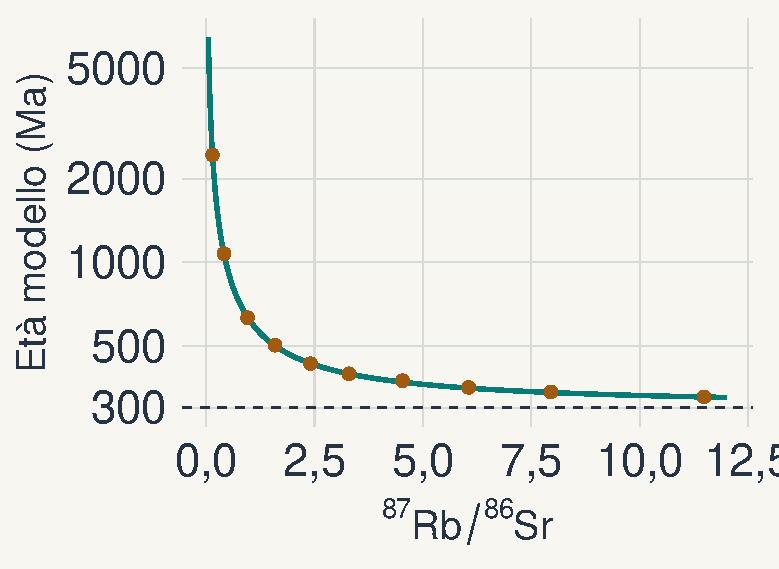
\includegraphics[width=\linewidth,height=6.15cm,keepaspectratio]{Figure/F01.pdf}\par}
\PSmall{Età modello con rapporto iniziale assunto 0,704, in scala logaritmica; punti: i dieci campioni del granito; tratteggio: 300 Ma.}
}};
\node[anchor=north west,inner sep=0] at([xshift=10.85cm,yshift=-2.12cm]current page.north west){\Colonna{8.16cm}{\PBody{Con un rapporto iniziale sottostimato di 0,0045, l’età modello di un campione con ${}^{87}$Rb/${}^{86}$Sr di 0,15 supera i due miliardi di anni; per il campione più ricco di rubidio, con rapporto 11,5, l’errore si riduce a 28 milioni di anni. L’errore sul rapporto iniziale si divide per ${}^{87}$Rb/${}^{86}$Sr.}
\PSmall{L’isocrona del capitolo successivo stima insieme età e rapporto iniziale.}
}};
\end{tikzpicture}\end{frame}

\begin{frame}[plain]\hypertarget{slide8}{}
\bookmark[level=1,page=8]{Età modello e rapporto iniziale}
\begin{tikzpicture}[remember picture,overlay]
\PilotChrome{Età modello e rapporto iniziale}{IL DECADIMENTO COME OROLOGIO}{8}{Valutare come un errore sul rapporto iniziale sposta l’età modello al variare di ${}^{87}$Rb/${}^{86}$Sr.}
\node[anchor=north west,inner sep=0] at([xshift=.96cm,yshift=-2.12cm]current page.north west){\Colonna{9.40cm}{{\centering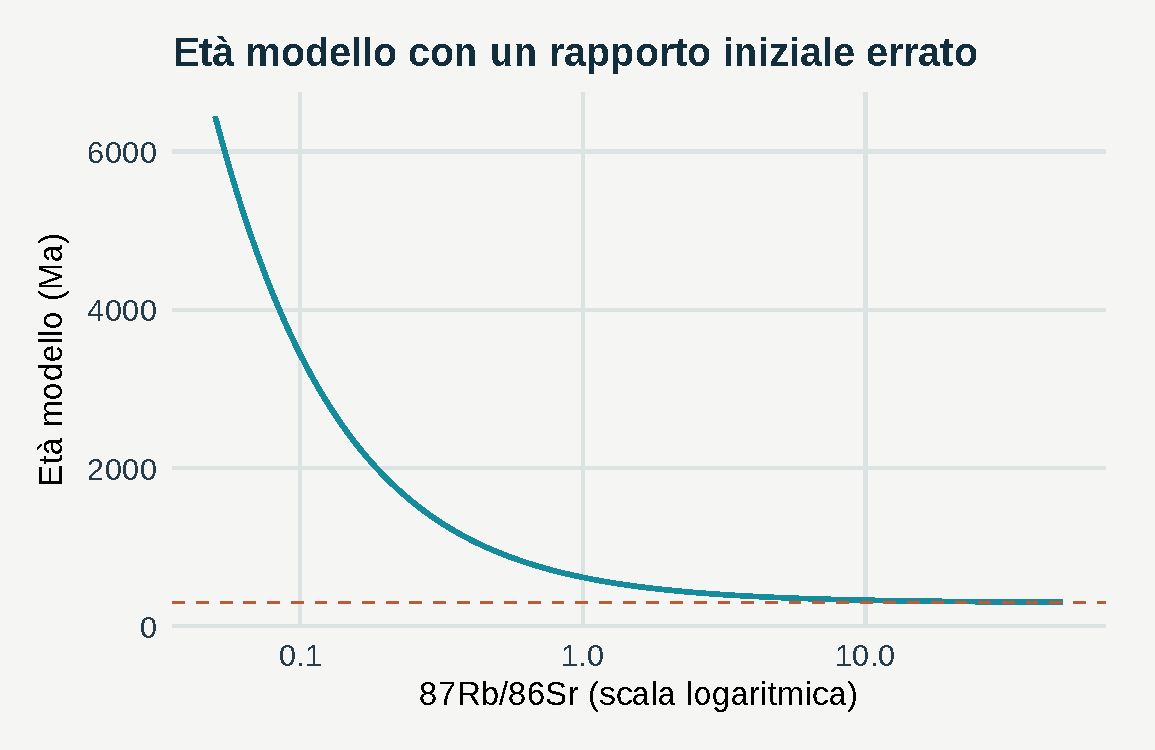
\includegraphics[width=\linewidth,height=6.0cm,keepaspectratio]{Esperimenti/m19-modello-A.pdf}\par}
\PSmall{Errore sul rapporto iniziale: 0,0045; età vera 300 Ma.}
}};
\node[anchor=north west,inner sep=0] at([xshift=10.85cm,yshift=-2.12cm]current page.north west){\Colonna{8.16cm}{\PLabel{Scenario A · simulazione}
\PBody{L’esperimento calcola le età modello di campioni con ${}^{87}$Rb/${}^{86}$Sr fra 0,05 e 50, generati senza errori di misura da un sistema con età e rapporto iniziale noti, usando un rapporto iniziale assunto più basso della quantità impostata.}
\par\smallskip{\centering\adjustbox{max width=.98\linewidth}{$\displaystyle t_{\mathrm{mod}}=\frac1\lambda\log\Big(1+\frac{y-r_0}{x}\Big)$}\par\smallskip}
\PSmall{$x$ e $y$ sono ${}^{87}$Rb/${}^{86}$Sr e ${}^{87}$Sr/${}^{86}$Sr; il calcolo è deterministico.}
}};
\node[anchor=north east,inner sep=0] at([xshift=17.1cm,yshift=-12.04cm]current page.north west){\fontsize{7.7}{9}\selectfont \href{https://marzione00.github.io/Lab_Geo/\#laboratorio/m19-modello}{\color{Classical}\bfseries Apri il laboratorio · m19-modello}};
\end{tikzpicture}\end{frame}

\begin{frame}[plain]\hypertarget{slide9}{}
\bookmark[level=1,page=9]{Confronto | Età modello e rapporto iniziale}
\begin{tikzpicture}[remember picture,overlay]
\PilotChrome{Confronto | Età modello e rapporto iniziale}{IL DECADIMENTO COME OROLOGIO}{9}{L’errore sull’età modello è circa proporzionale all’errore sul rapporto iniziale.}
\node[anchor=north west,inner sep=0] at([xshift=.96cm,yshift=-2.12cm]current page.north west){\Colonna{9.40cm}{{\centering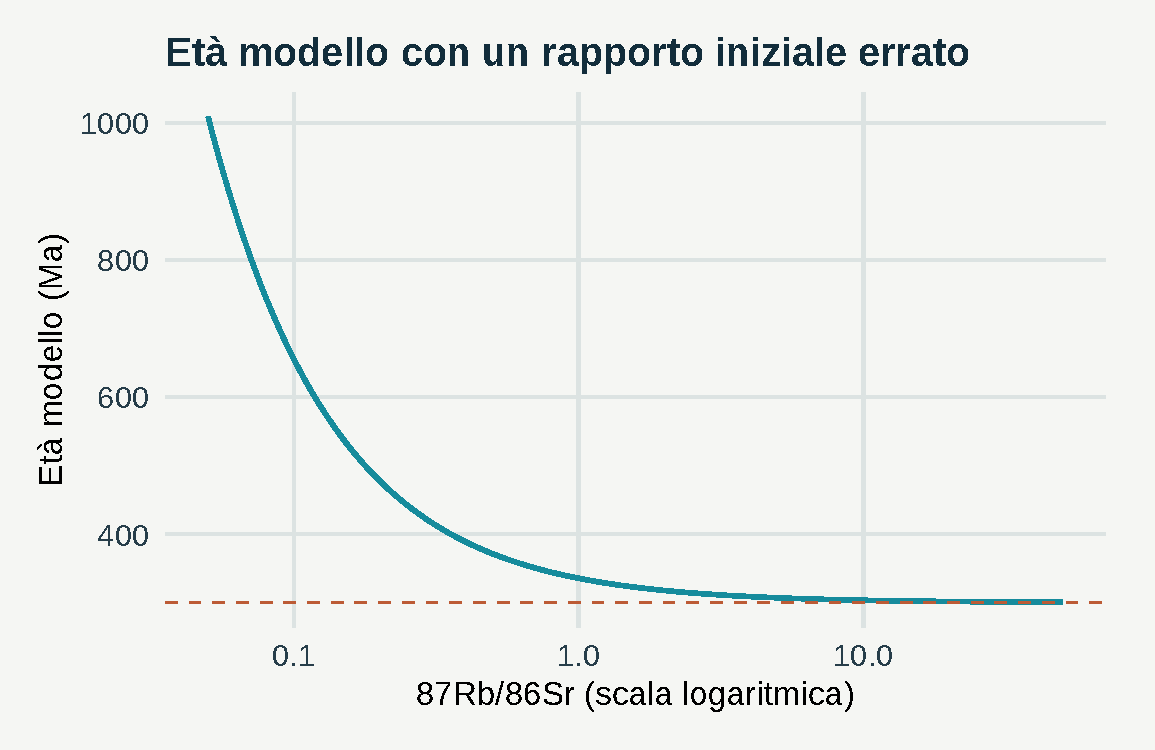
\includegraphics[width=\linewidth,height=5.6cm,keepaspectratio]{Esperimenti/m19-modello-B.pdf}\par}
\PSmall{Errore sul rapporto iniziale: 0,0045 $\to$ 0,0005. L’età vera resta 300 Ma.}
}};
\node[anchor=north west,inner sep=0] at([xshift=10.85cm,yshift=-2.12cm]current page.north west){\Colonna{8.16cm}{\PLabel{Confronto fra gli scenari}
{\fontsize{10.2}{12.8}\selectfont\begin{tabular}{@{}>{\raggedright\arraybackslash}p{0.48\linewidth}@{\hspace{.13cm}}>{\raggedright\arraybackslash}p{0.224\linewidth}@{\hspace{.13cm}}>{\raggedright\arraybackslash}p{0.224\linewidth}@{}}\toprule Grandezza & A & B\\[2.3pt]
\midrule 
Età vera (Ma) & 300 & 300\\[2.3pt]
Età modello, $x=0{,}5$ & 939 & 371\\[2.3pt]
Età modello, $x=5$ & 364 & 307\\[2.3pt]
Età modello, $x=50$ & 306 & 301\\[2.3pt]
\bottomrule\end{tabular}\par}
\vspace{.25cm}\PBody{Con un errore di 0,0005 l’età modello di un campione con rapporto 0,5 scende da 939 a 371 milioni di anni; per un rapporto 50 resta entro 1 milione di anni dal valore vero.}
}};
\node[anchor=north east,inner sep=0] at([xshift=17.1cm,yshift=-12.04cm]current page.north west){\fontsize{7.7}{9}\selectfont \href{https://marzione00.github.io/Lab_Geo/\#laboratorio/m19-modello}{\color{Classical}\bfseries Apri il laboratorio · m19-modello}};
\end{tikzpicture}\end{frame}

\begin{frame}[plain]\hypertarget{slide10}{}
\bookmark[level=0,page=10]{L’isocrona}
\bookmark[level=1,page=10]{Campioni coevi stanno su una retta}
\begin{tikzpicture}[remember picture,overlay]
\PilotChrome{Campioni coevi stanno su una retta}{L’ISOCRONA}{10}{La pendenza dell’isocrona dà l’età, l’intercetta il rapporto iniziale.}
\node[anchor=north west,inner sep=0] at([xshift=.96cm,yshift=-2.12cm]current page.north west){\Colonna{9.40cm}{{\centering\resizebox{0.94\linewidth}{!}{\begin{tikzpicture}[x=1cm,y=1cm,every node/.append style={anchor=center,inner sep=.3333em}]
\draw[-{Latex[length=2mm]},Ink,line width=.6pt] (0,0)--(7.2,0) node[pNote,anchor=north east,yshift=-1mm]{${}^{87}$Rb/${}^{86}$Sr};
\draw[-{Latex[length=2mm]},Ink,line width=.6pt] (0,0)--(0,4.3) node[pNote,anchor=south]{${}^{87}$Sr/${}^{86}$Sr};
\draw[Muted,line width=1pt] (0,1)--(6.6,1);
\draw[GeoA,line width=1.3pt] (0,1)--(6.6,3.7);
\foreach \x in {1.2,2.6,4.1,5.8}{
 \fill[Muted] (\x,1) circle(2pt);
 \fill[GeoA] (\x,{1+\x*2.7/6.6}) circle(2.4pt);
 \draw[-{Latex[length=1.6mm]},GeoB,line width=.7pt] (\x,1.08)--(\x,{0.94+\x*2.7/6.6});}
\fill[Ink] (0,1) circle(2.2pt) node[pNote,anchor=east]{$r_0$\ };
\node[pLabel,text=Muted,anchor=west] at(6.65,1){$t=0$};
\node[pLabel,text=GeoA,anchor=west] at(6.65,3.7){oggi};
\node[pNote,text width=7.2cm] at(3.4,-1.05){Ogni campione sale in proporzione al suo ${}^{87}$Rb/${}^{86}$Sr: i punti restano allineati e la retta ruota attorno a $r_0$, con pendenza $e^{\lambda t}-1$.};
\end{tikzpicture}
}\par}
\PSmall{Campioni con lo stesso rapporto iniziale, alla formazione e oggi.}
}};
\node[anchor=north west,inner sep=0] at([xshift=10.85cm,yshift=-2.12cm]current page.north west){\Colonna{8.16cm}{\PBody{Minerali e rocce che si formano insieme dallo stesso fuso hanno lo stesso ${}^{87}$Sr/${}^{86}$Sr e rapporti ${}^{87}$Rb/${}^{86}$Sr diversi. Con il tempo ogni campione aumenta il suo ${}^{87}$Sr/${}^{86}$Sr in proporzione al rubidio che contiene: i punti restano su una retta che ruota attorno al rapporto iniziale.}
\par\smallskip{\centering\adjustbox{max width=.98\linewidth}{$\displaystyle y=r_0+\big(e^{\lambda t}-1\big)\,x$}\par\smallskip}
\PSmall{Dalla pendenza $b$ l’età si ottiene come $t=\log(1+b)/\lambda$.}
}};
\end{tikzpicture}\end{frame}

\begin{frame}[plain]\hypertarget{slide11}{}
\bookmark[level=1,page=11]{L’isocrona del granito}
\begin{tikzpicture}[remember picture,overlay]
\PilotChrome{L’isocrona del granito}{L’ISOCRONA}{11}{Un’isocrona richiede campioni coevi, cogenetici e rimasti sistemi chiusi.}
\node[anchor=north west,inner sep=0] at([xshift=.96cm,yshift=-2.12cm]current page.north west){\Colonna{9.40cm}{{\centering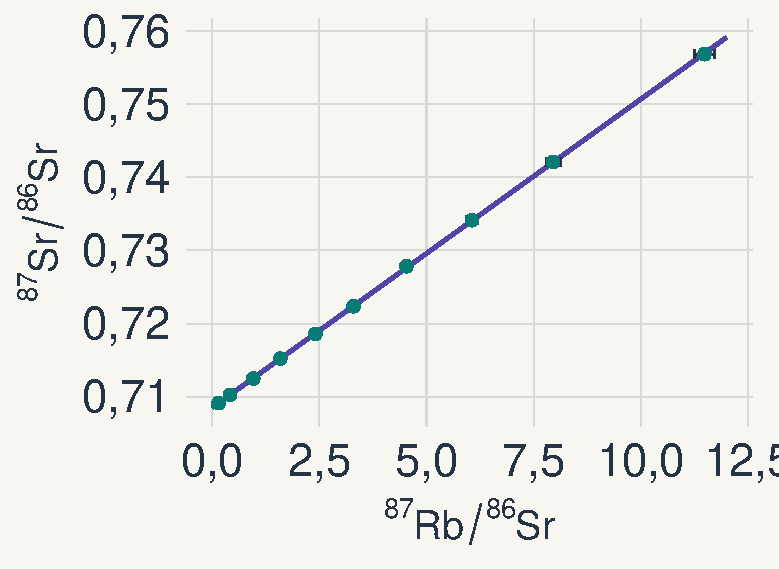
\includegraphics[width=\linewidth,height=6.15cm,keepaspectratio]{Figure/F02.pdf}\par}
\PSmall{Dieci campioni del granito con barre di due deviazioni standard su ${}^{87}$Rb/${}^{86}$Sr e la retta di York.}
}};
\node[anchor=north west,inner sep=0] at([xshift=10.85cm,yshift=-2.12cm]current page.north west){\Colonna{8.16cm}{\PBody{I dieci campioni del granito hanno ${}^{87}$Rb/${}^{86}$Sr fra 0,15 e 11,5. Le incertezze dichiarate sono dell’1\% su ${}^{87}$Rb/${}^{86}$Sr e di $1{,}1\cdot10^{-5}$ su ${}^{87}$Sr/${}^{86}$Sr: le barre verticali sono più piccole dei simboli. I punti sono allineati entro gli errori, e la retta stima insieme età e rapporto iniziale.}
\PSmall{La correlazione fra gli errori dei due rapporti è posta a zero nel file del caso.}
}};
\end{tikzpicture}\end{frame}

\begin{frame}[plain]\hypertarget{slide12}{}
\bookmark[level=1,page=12]{La retta dei minimi quadrati ordinari}
\begin{tikzpicture}[remember picture,overlay]
\PilotChrome{La retta dei minimi quadrati ordinari}{L’ISOCRONA}{12}{I minimi quadrati ordinari ignorano le incertezze dichiarate dei campioni.}
\node[anchor=north west,inner sep=0] at([xshift=.96cm,yshift=-2.12cm]current page.north west){\Colonna{9.40cm}{\PBody{Il codice adatta una retta con \texttt{lm}: pendenza 0,0042129, rapporto iniziale 0,70852, età 300,9 milioni di anni. Il metodo tratta ${}^{87}$Rb/${}^{86}$Sr come noto senza errore, dà lo stesso peso a tutti i campioni e stima la dispersione dai residui: le incertezze analitiche dichiarate non entrano nel calcolo.}
\par\smallskip{\centering\adjustbox{max width=.98\linewidth}{$\displaystyle \min_{a,b}\sum_i\big(y_i-a-bx_i\big)^2$}\par\smallskip}
}};
\node[anchor=north west,inner sep=0] at([xshift=10.85cm,yshift=-2.12cm]current page.north west){\Colonna{8.16cm}{\begin{tcolorbox}[enhanced,arc=1.7mm,boxrule=.6pt,colback=white,colframe=Classical!60!Navy,colbacktitle=Navy,coltitle=white,fonttitle=\bfseries\small,title={R · calcolo riproducibile},left=1.7mm,right=1.3mm,top=1.1mm,bottom=1.1mm,before skip=1mm,after skip=1.0mm]\lstinputlisting[style=GeoR,language=R]{Codice/capitolo-03.R}\end{tcolorbox}
\PLabel{Risultato in R}
\begin{tcolorbox}[colback=GeoTint,colframe=Rule,boxrule=.5pt,arc=1.4mm,left=2mm,right=1mm,top=1mm,bottom=1mm]{\fontsize{8.6}{11.4}\selectfont\ttfamily \mbox{\ iniziale\ \ pendenza\ \ \ \ eta\_Ma}\\\mbox{\ \ 0.70852\ \ \ 0.00421\ 300.89323}}\end{tcolorbox}}};
\end{tikzpicture}\end{frame}

\begin{frame}[plain]\hypertarget{slide13}{}
\bookmark[level=1,page=13]{Errori su entrambi gli assi}
\begin{tikzpicture}[remember picture,overlay]
\PilotChrome{Errori su entrambi gli assi}{L’ISOCRONA}{13}{La regressione di York minimizza la somma dei residui pesati con gli errori dei due rapporti.}
\node[anchor=north west,inner sep=0] at([xshift=.96cm,yshift=-2.12cm]current page.north west){\Colonna{9.40cm}{{\centering\resizebox{0.94\linewidth}{!}{\begin{tikzpicture}[x=1cm,y=1cm,every node/.append style={anchor=center,inner sep=.3333em}]
\draw[GeoA,line width=1.2pt] (-.4,-.2)--(6.4,3.2);
\coordinate (P) at (2.2,2.5);
\coordinate (Q) at (3.25,1.625);
\draw[GeoB,line width=.8pt,fill=GeoB!10] (P) ellipse(1.15 and .32);
\fill[Ink] (P) circle(2.2pt) node[pLabel,anchor=south,yshift=2.4mm]{$(X_i,Y_i)$};
\draw[-{Latex[length=2mm]},Classical,line width=.9pt] (P)--(Q);
\fill[Classical] (Q) circle(2pt) node[pNote,anchor=north west,text=Classical]{punto corretto};
\draw[Muted,dashed] (P)--(2.2,1.1);
\node[pNote,text=Muted,anchor=east] at(2.15,1.75){residuo verticale};
\node[pNote,text width=7.4cm] at(3,-1.2){L’ellisse rappresenta gli errori del campione: ampia in orizzontale, stretta in verticale. York sposta il punto sulla retta nella direzione più compatibile con i suoi errori e pesa ciascun residuo con $W_i$.};
\end{tikzpicture}
}\par}
\PSmall{Un campione, la sua ellisse di errore e il punto corretto sulla retta.}
}};
\node[anchor=north west,inner sep=0] at([xshift=10.85cm,yshift=-2.12cm]current page.north west){\Colonna{8.16cm}{\PBody{Derek York e colleghi pubblicarono nel 2004 equazioni unificate per la retta con errori su $x$ e $y$, anche correlati. Ogni campione riceve un peso $W_i$ che combina i due errori secondo la pendenza; l’algoritmo aggiorna pendenza e pesi fino alla convergenza e calcola gli errori standard nei punti corretti.}
\par\smallskip{\centering\adjustbox{max width=.98\linewidth}{$\displaystyle W_i=\frac{\omega(X_i)\,\omega(Y_i)}{\omega(X_i)+b^2\,\omega(Y_i)},\qquad \omega=\frac1{\sigma^2}$}\par\smallskip}
}};
\end{tikzpicture}\end{frame}

\begin{frame}[plain]\hypertarget{slide14}{}
\bookmark[level=1,page=14]{La retta di York del granito}
\begin{tikzpicture}[remember picture,overlay]
\PilotChrome{La retta di York del granito}{L’ISOCRONA}{14}{L’errore standard dell’età si ottiene da quello della pendenza.}
\node[anchor=north west,inner sep=0] at([xshift=.96cm,yshift=-2.12cm]current page.north west){\Colonna{9.40cm}{\PBody{La funzione \texttt{york} in \texttt{R/york.R} applica l’algoritmo. Per il granito la pendenza vale $0{,}0042158\pm0{,}0000166$, il rapporto iniziale $0{,}708506\pm0{,}000012$ e l’età $301{,}1\pm1{,}2$ milioni di anni, con MSWD 0,50. Su duemila isocrone simulate la deviazione standard delle pendenze è $1{,}64\cdot10^{-5}$.}
\par\smallskip{\centering\adjustbox{max width=.98\linewidth}{$\displaystyle \sigma_t=\frac{\sigma_b}{\lambda\,(1+b)}$}\par\smallskip}
}};
\node[anchor=north west,inner sep=0] at([xshift=10.85cm,yshift=-2.12cm]current page.north west){\Colonna{8.16cm}{\begin{tcolorbox}[enhanced,arc=1.7mm,boxrule=.6pt,colback=white,colframe=Classical!60!Navy,colbacktitle=Navy,coltitle=white,fonttitle=\bfseries\small,title={R · calcolo riproducibile},left=1.7mm,right=1.3mm,top=1.1mm,bottom=1.1mm,before skip=1mm,after skip=1.0mm]\lstinputlisting[style=GeoR,language=R]{Codice/capitolo-04.R}\end{tcolorbox}
\PLabel{Risultato in R}
\begin{tcolorbox}[colback=GeoTint,colframe=Rule,boxrule=.5pt,arc=1.4mm,left=2mm,right=1mm,top=1mm,bottom=1mm]{\fontsize{8.6}{11.4}\selectfont\ttfamily \mbox{\ \ \ \ \ \ \ \ a\ \ \ \ \ \ \ \ sa\ \ \ \ \ \ \ \ \ b\ \ \ \ \ \ \ \ sb}\\\mbox{0.7085063\ 0.0000119\ 0.0042158\ 0.0000166}\\\mbox{\ \ \ mswd\ \ \ \ \ eta\ \ \ s\_eta}\\\mbox{\ \ 0.503\ 301.101\ \ \ 1.180}}\end{tcolorbox}}};
\end{tikzpicture}\end{frame}

\begin{frame}[plain]\hypertarget{slide15}{}
\bookmark[level=1,page=15]{Minimi quadrati ordinari e regressione di York}
\begin{tikzpicture}[remember picture,overlay]
\PilotChrome{Minimi quadrati ordinari e regressione di York}{L’ISOCRONA}{15}{Confrontare le età dei due metodi quando anche ${}^{87}$Rb/${}^{86}$Sr ha errori di misura.}
\node[anchor=north west,inner sep=0] at([xshift=.96cm,yshift=-2.12cm]current page.north west){\Colonna{9.40cm}{{\centering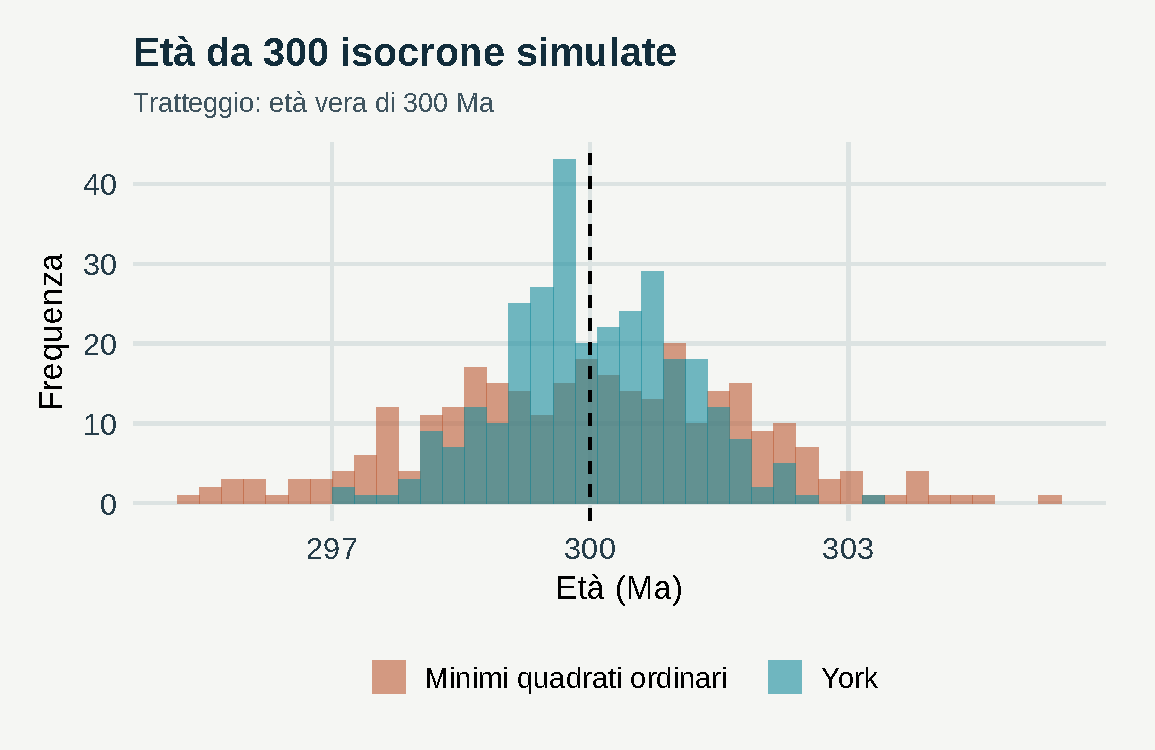
\includegraphics[width=\linewidth,height=6.0cm,keepaspectratio]{Esperimenti/m19-york-A.pdf}\par}
\PSmall{Errore relativo su ${}^{87}$Rb/${}^{86}$Sr: 1\%; dieci campioni. Seme: 17.}
}};
\node[anchor=north west,inner sep=0] at([xshift=10.85cm,yshift=-2.12cm]current page.north west){\Colonna{8.16cm}{\PLabel{Scenario A · simulazione}
\PBody{L’esperimento simula trecento isocrone di un sistema di 300 milioni di anni e calcola l’età con i minimi quadrati ordinari e con la regressione di York. Con errori dell’1\% le due età medie coincidono; la deviazione standard è 1,82 milioni di anni con i minimi quadrati e 1,03 con York.}
\par\smallskip{\centering\adjustbox{max width=.98\linewidth}{$\displaystyle \hat t=\frac{\log(1+\hat b)}{\lambda}$}\par\smallskip}
\PSmall{$\hat b$ è la pendenza stimata in ciascuna isocrona simulata.}
}};
\node[anchor=north east,inner sep=0] at([xshift=17.1cm,yshift=-12.04cm]current page.north west){\fontsize{7.7}{9}\selectfont \href{https://marzione00.github.io/Lab_Geo/\#laboratorio/m19-york}{\color{Classical}\bfseries Apri il laboratorio · m19-york}};
\end{tikzpicture}\end{frame}

\begin{frame}[plain]\hypertarget{slide16}{}
\bookmark[level=1,page=16]{Confronto | Minimi quadrati ordinari e York}
\begin{tikzpicture}[remember picture,overlay]
\PilotChrome{Confronto | Minimi quadrati ordinari e York}{L’ISOCRONA}{16}{Errori grandi sull’asse orizzontale rendono i minimi quadrati ordinari distorti verso il basso.}
\node[anchor=north west,inner sep=0] at([xshift=.96cm,yshift=-2.12cm]current page.north west){\Colonna{9.40cm}{{\centering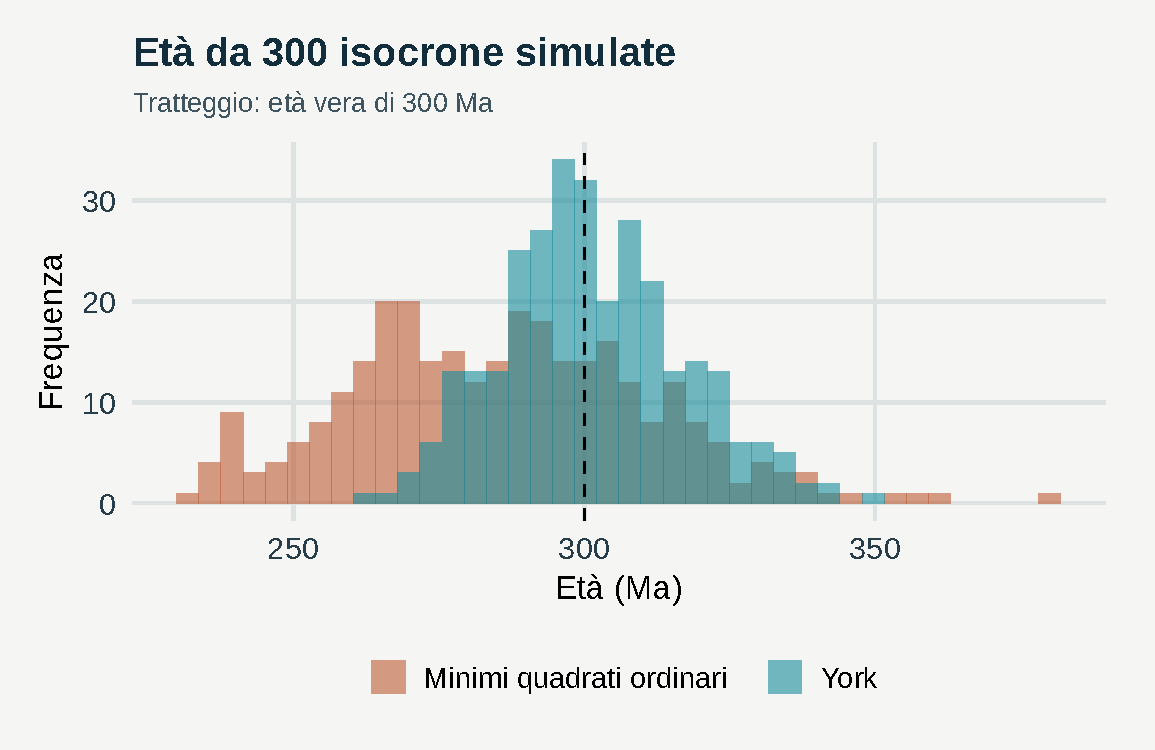
\includegraphics[width=\linewidth,height=5.6cm,keepaspectratio]{Esperimenti/m19-york-B.pdf}\par}
\PSmall{Errore relativo su ${}^{87}$Rb/${}^{86}$Sr: 1 $\to$ 15\%. Tutti gli altri parametri e il seme sono fissi.}
}};
\node[anchor=north west,inner sep=0] at([xshift=10.85cm,yshift=-2.12cm]current page.north west){\Colonna{8.16cm}{\PLabel{Confronto fra gli scenari}
{\fontsize{10.2}{12.8}\selectfont\begin{tabular}{@{}>{\raggedright\arraybackslash}p{0.48\linewidth}@{\hspace{.13cm}}>{\raggedright\arraybackslash}p{0.224\linewidth}@{\hspace{.13cm}}>{\raggedright\arraybackslash}p{0.224\linewidth}@{}}\toprule Grandezza & A & B\\[2.3pt]
\midrule 
Età media, minimi quadrati & 300 & 286\\[2.3pt]
Età media, York & 300 & 301\\[2.3pt]
Dev. standard, minimi quadrati & 1{,}82 & 25{,}8\\[2.3pt]
Dev. standard, York & 1{,}03 & 15{,}6\\[2.3pt]
\bottomrule\end{tabular}\par}
\vspace{.25cm}\PBody{Con errori del 15\% l’età media dei minimi quadrati scende a 286 milioni di anni; quella di York resta vicina a 300, con una dispersione minore.}
}};
\node[anchor=north east,inner sep=0] at([xshift=17.1cm,yshift=-12.04cm]current page.north west){\fontsize{7.7}{9}\selectfont \href{https://marzione00.github.io/Lab_Geo/\#laboratorio/m19-york}{\color{Classical}\bfseries Apri il laboratorio · m19-york}};
\end{tikzpicture}\end{frame}

\begin{frame}[plain]\hypertarget{slide17}{}
\bookmark[level=0,page=17]{MSWD e dispersione in eccesso}
\bookmark[level=1,page=17]{Che valori può avere la MSWD}
\begin{tikzpicture}[remember picture,overlay]
\PilotChrome{Che valori può avere la MSWD}{MSWD E DISPERSIONE IN ECCESSO}{17}{La MSWD vale in media 1 se gli errori dichiarati descrivono la dispersione; la sua variabilità dipende da $f$.}
\node[anchor=north west,inner sep=0] at([xshift=.96cm,yshift=-2.12cm]current page.north west){\Colonna{9.40cm}{{\centering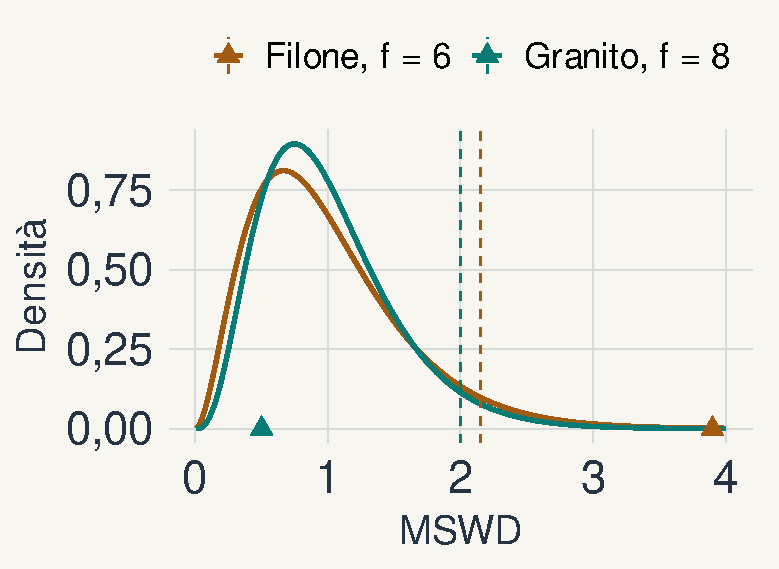
\includegraphics[width=\linewidth,height=6.15cm,keepaspectratio]{Figure/F03.pdf}\par}
\PSmall{Distribuzioni della MSWD per 8 e 6 gradi di libertà, soglie di Wendt e Carl (tratteggio) e valori osservati (triangoli).}
}};
\node[anchor=north west,inner sep=0] at([xshift=10.85cm,yshift=-2.12cm]current page.north west){\Colonna{8.16cm}{\PBody{La MSWD è la somma dei residui pesati al quadrato divisa per i gradi di libertà $f=n-2$. I. Wendt e C. Carl mostrarono nel 1991 che il suo valore atteso è 1 per ogni $f$ e la sua deviazione standard $\sqrt{2/f}$; un valore oltre $1+2\sqrt{2/f}$ ha probabilità inferiore al 5\%. Il granito ha MSWD 0,50 con soglia 2,00; il filone 3,94 con soglia 2,15.}
\par\smallskip{\centering\adjustbox{max width=.98\linewidth}{$\displaystyle \mathrm{MSWD}=\frac{1}{f}\sum_{i=1}^n W_i\big(Y_i-a-bX_i\big)^2$}\par\smallskip}
}};
\end{tikzpicture}\end{frame}

\begin{frame}[plain]\hypertarget{slide18}{}
\bookmark[level=1,page=18]{I campioni del filone formano un’isocrona?}
\begin{tikzpicture}[remember picture,overlay]
\PilotChrome{I campioni del filone formano un’isocrona?}{MSWD E DISPERSIONE IN ECCESSO}{18}{Una MSWD oltre la soglia indica una dispersione che gli errori analitici non spiegano.}
\node[anchor=north west,inner sep=0] at([xshift=.96cm,yshift=-2.12cm]current page.north west){\Colonna{9.40cm}{\PLabel{Domanda}
\PBody{Gli otto campioni del filone hanno le stesse incertezze analitiche del granito. La loro dispersione attorno alla retta di York è compatibile con quelle incertezze?}
\vspace{.35cm}\PLabel{Interpretazione}
\PBody{La MSWD vale 3,94 con sei gradi di libertà, oltre la soglia di 2,15; la probabilità di un valore così grande con i soli errori analitici è 0,0006. I campioni del filone hanno una dispersione in eccesso.}
}};
\node[anchor=north west,inner sep=0] at([xshift=10.85cm,yshift=-2.12cm]current page.north west){\Colonna{8.16cm}{\begin{tcolorbox}[enhanced,arc=1.7mm,boxrule=.6pt,colback=white,colframe=Classical!60!Navy,colbacktitle=Navy,coltitle=white,fonttitle=\bfseries\small,title={R · calcolo riproducibile},left=1.7mm,right=1.3mm,top=1.1mm,bottom=1.1mm,before skip=1mm,after skip=1.0mm]\lstinputlisting[style=GeoR,language=R]{Codice/capitolo-05.R}\end{tcolorbox}
\PLabel{Risultato in R}
\begin{tcolorbox}[colback=GeoTint,colframe=Rule,boxrule=.5pt,arc=1.4mm,left=2mm,right=1mm,top=1mm,bottom=1mm]{\fontsize{8.6}{11.4}\selectfont\ttfamily \mbox{\ \ mswd\ soglia\ \ \ \ \ \ p}\\\mbox{3.9374\ 2.1547\ 0.0006}}\end{tcolorbox}}};
\end{tikzpicture}\end{frame}

\begin{frame}[plain]\hypertarget{slide19}{}
\bookmark[level=1,page=19]{Dove sta la dispersione in eccesso}
\begin{tikzpicture}[remember picture,overlay]
\PilotChrome{Dove sta la dispersione in eccesso}{MSWD E DISPERSIONE IN ECCESSO}{19}{I residui pesati si leggono in unità di deviazione standard: oltre $\pm2$ sono rari se gli errori sono corretti.}
\node[anchor=north west,inner sep=0] at([xshift=.96cm,yshift=-2.12cm]current page.north west){\Colonna{9.40cm}{{\centering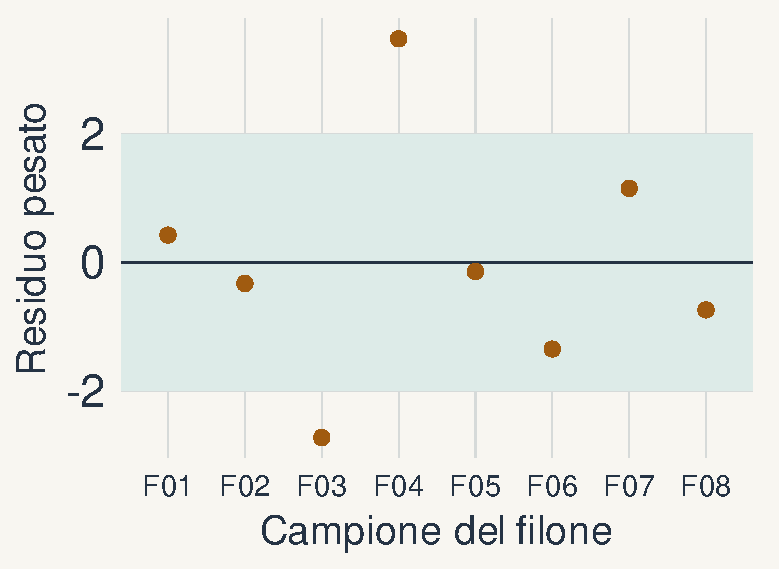
\includegraphics[width=\linewidth,height=6.15cm,keepaspectratio]{Figure/F04.pdf}\par}
\PSmall{Residui pesati degli otto campioni del filone rispetto alla retta di York; fascia: $\pm2$.}
}};
\node[anchor=north west,inner sep=0] at([xshift=10.85cm,yshift=-2.12cm]current page.north west){\Colonna{8.16cm}{\PBody{Il residuo pesato divide lo scarto verticale dalla retta per la sua deviazione standard combinata. Due campioni, F03 e F04, hanno residui di $-2{,}73$ e $+3{,}49$; gli altri restano entro $\pm1{,}4$. Nel generatore il rapporto iniziale del filone varia da campione a campione, come in un fuso non omogeneo.}
\par\smallskip{\centering\adjustbox{max width=.98\linewidth}{$\displaystyle e_i=\big(Y_i-a-bX_i\big)\sqrt{W_i}$}\par\smallskip}
}};
\end{tikzpicture}\end{frame}

\begin{frame}[plain]\hypertarget{slide20}{}
\bookmark[level=1,page=20]{Scalare l’incertezza con la MSWD}
\begin{tikzpicture}[remember picture,overlay]
\PilotChrome{Scalare l’incertezza con la MSWD}{MSWD E DISPERSIONE IN ECCESSO}{20}{Scalare per $\sqrt{\mathrm{MSWD}}$ presuppone una dispersione in eccesso proporzionale agli errori analitici.}
\node[anchor=north west,inner sep=0] at([xshift=.96cm,yshift=-2.12cm]current page.north west){\Colonna{9.40cm}{\PBody{Una pratica diffusa moltiplica l’errore standard per la radice della MSWD, attribuendo l’eccesso a errori analitici sottostimati in modo uniforme. Per il filone l’età è 247,5 milioni di anni; l’incertezza passa da 1,23 a 2,44 milioni di anni. Il valore del generatore, 250, cade entro due incertezze scalate.}
\par\smallskip{\centering\adjustbox{max width=.98\linewidth}{$\displaystyle \sigma_t^{*}=\sigma_t\sqrt{\mathrm{MSWD}}$}\par\smallskip}
}};
\node[anchor=north west,inner sep=0] at([xshift=10.85cm,yshift=-2.12cm]current page.north west){\Colonna{8.16cm}{\begin{tcolorbox}[enhanced,arc=1.7mm,boxrule=.6pt,colback=white,colframe=Classical!60!Navy,colbacktitle=Navy,coltitle=white,fonttitle=\bfseries\small,title={R · calcolo riproducibile},left=1.7mm,right=1.3mm,top=1.1mm,bottom=1.1mm,before skip=1mm,after skip=1.0mm]\lstinputlisting[style=GeoR,language=R]{Codice/capitolo-06.R}\end{tcolorbox}
\PLabel{Risultato in R}
\begin{tcolorbox}[colback=GeoTint,colframe=Rule,boxrule=.5pt,arc=1.4mm,left=2mm,right=1mm,top=1mm,bottom=1mm]{\fontsize{8.6}{11.4}\selectfont\ttfamily \mbox{\ \ \ \ \ \ eta\ \ \ \ \ \ \ \ \ s\ s\_scalato}\\\mbox{\ \ \ 247.54\ \ \ \ \ \ 1.23\ \ \ \ \ \ 2.44}}\end{tcolorbox}}};
\end{tikzpicture}\end{frame}

\begin{frame}[plain]\hypertarget{slide21}{}
\bookmark[level=1,page=21]{Che cosa può significare una MSWD lontana da 1}
\begin{tikzpicture}[remember picture,overlay]
\PilotChrome{Che cosa può significare una MSWD lontana da 1}{MSWD E DISPERSIONE IN ECCESSO}{21}{Una MSWD vicina a 1 è compatibile con il modello; da sola non lo conferma.}
\node[anchor=north west,inner sep=0] at([xshift=.96cm,yshift=-2.12cm]current page.north west){\Colonna{9.40cm}{\PLabel{MSWD grande}
\PBody{Una MSWD oltre la soglia può nascere da errori analitici sottostimati o da una dispersione geologica: rapporti iniziali diversi, sistemi aperti dopo la formazione, campioni di età diverse. Le due spiegazioni portano a modelli diversi, e la scelta richiede informazioni geologiche oltre al valore della statistica.}
}};
\node[anchor=north west,inner sep=0] at([xshift=10.85cm,yshift=-2.12cm]current page.north west){\Colonna{8.16cm}{\PLabel{MSWD piccola}
\PBody{Pieter Vermeesch ha osservato nel 2025 che una MSWD piccola merita altrettanta attenzione: può indicare errori sovrastimati o un campione troppo piccolo per rivelare una dispersione reale. Raccomanda di quantificare la dispersione e scoraggia l’esclusione di dati al solo scopo di ridurre la MSWD.}
\PSmall{Nel granito la MSWD di 0,50 ha probabilità di coda 0,855: un valore comune con otto gradi di libertà.}
}};
\end{tikzpicture}\end{frame}

\begin{frame}[plain]\hypertarget{slide22}{}
\bookmark[level=1,page=22]{MSWD con errori sottostimati}
\begin{tikzpicture}[remember picture,overlay]
\PilotChrome{MSWD con errori sottostimati}{MSWD E DISPERSIONE IN ECCESSO}{22}{Osservare la MSWD quando gli errori dichiarati sono corretti e quando sono troppo piccoli.}
\node[anchor=north west,inner sep=0] at([xshift=.96cm,yshift=-2.12cm]current page.north west){\Colonna{9.40cm}{{\centering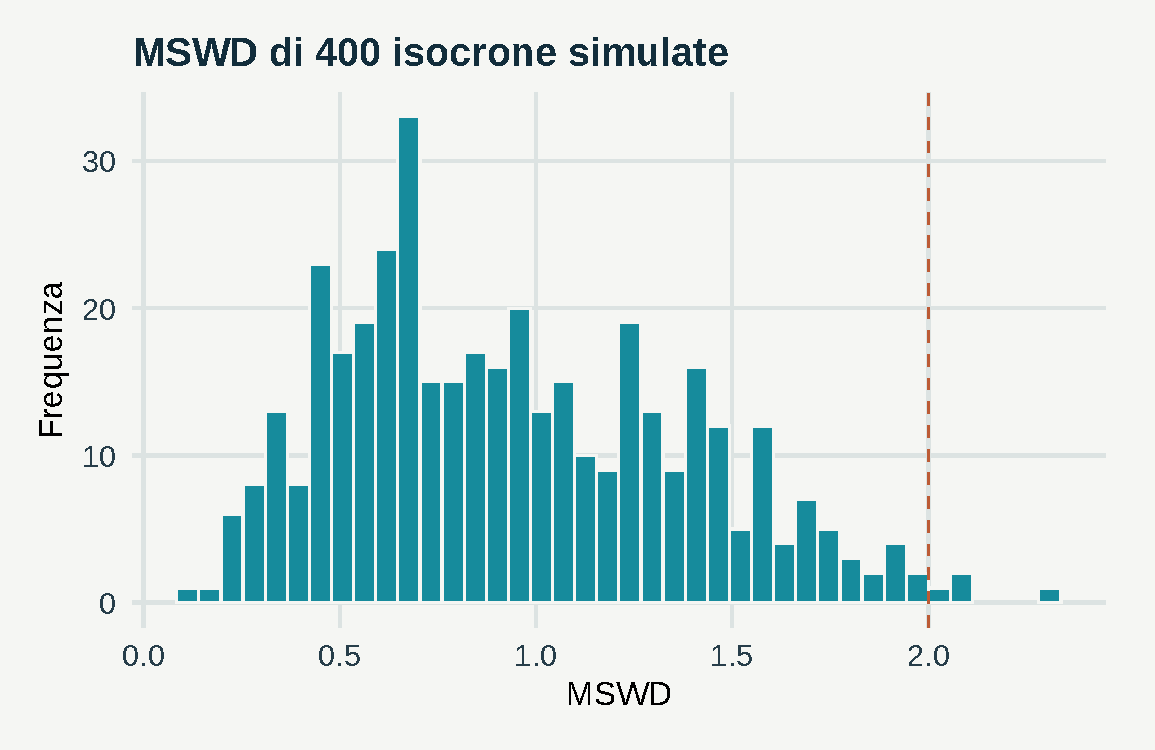
\includegraphics[width=\linewidth,height=6.0cm,keepaspectratio]{Esperimenti/m19-mswd-A.pdf}\par}
\PSmall{Errori reali uguali a quelli dichiarati; dieci campioni; quattrocento isocrone. Seme: 17.}
}};
\node[anchor=north west,inner sep=0] at([xshift=10.85cm,yshift=-2.12cm]current page.north west){\Colonna{8.16cm}{\PLabel{Scenario A · simulazione}
\PBody{L’esperimento simula quattrocento isocrone con errori reali pari agli errori dichiarati moltiplicati per un fattore. Con fattore 1 la MSWD media è 0,94 e l’intervallo di due errori standard contiene l’età vera nel 95,5\% dei casi.}
\par\smallskip{\centering\adjustbox{max width=.98\linewidth}{$\displaystyle E[\mathrm{MSWD}]=k^2$}\par\smallskip}
\PSmall{$k$ è il rapporto fra errori reali ed errori dichiarati; con molte simulazioni la quota oltre la soglia è circa il 4\%.}
}};
\node[anchor=north east,inner sep=0] at([xshift=17.1cm,yshift=-12.04cm]current page.north west){\fontsize{7.7}{9}\selectfont \href{https://marzione00.github.io/Lab_Geo/\#laboratorio/m19-mswd}{\color{Classical}\bfseries Apri il laboratorio · m19-mswd}};
\end{tikzpicture}\end{frame}

\begin{frame}[plain]\hypertarget{slide23}{}
\bookmark[level=1,page=23]{Confronto | MSWD con errori sottostimati}
\begin{tikzpicture}[remember picture,overlay]
\PilotChrome{Confronto | MSWD con errori sottostimati}{MSWD E DISPERSIONE IN ECCESSO}{23}{Errori dichiarati troppo piccoli producono intervalli di confidenza troppo stretti.}
\node[anchor=north west,inner sep=0] at([xshift=.96cm,yshift=-2.12cm]current page.north west){\Colonna{9.40cm}{{\centering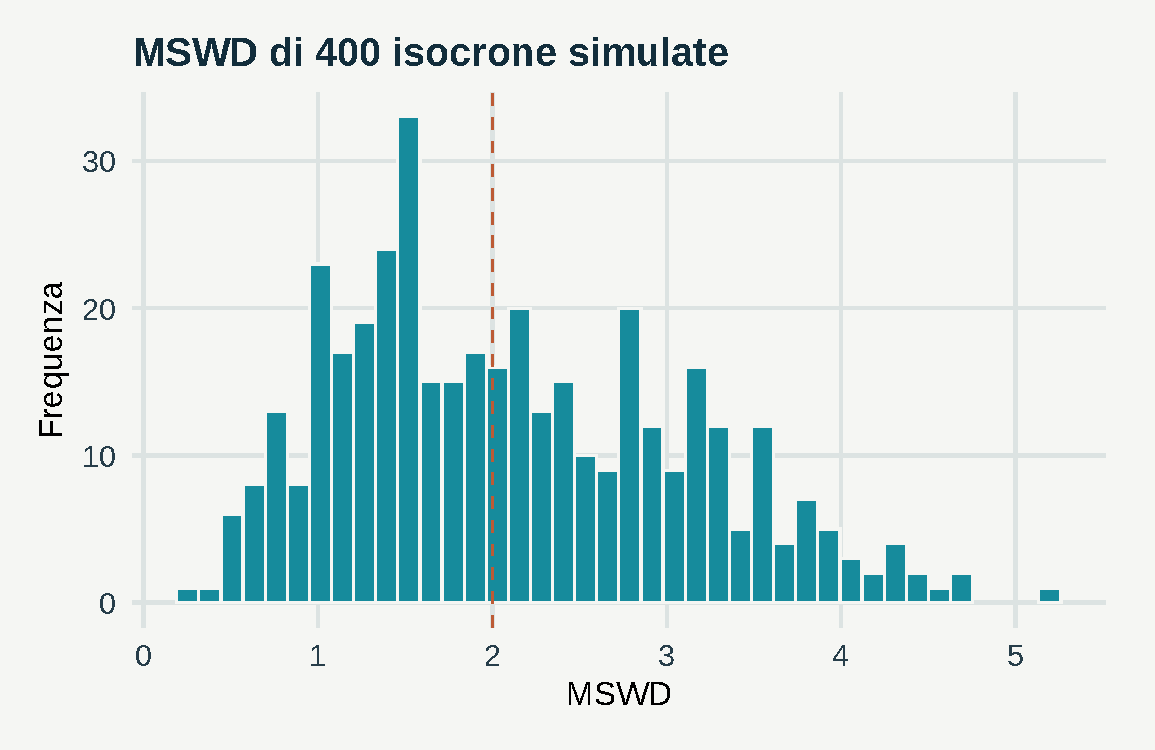
\includegraphics[width=\linewidth,height=5.6cm,keepaspectratio]{Esperimenti/m19-mswd-B.pdf}\par}
\PSmall{Errori reali / dichiarati: 1 $\to$ 1,5. Tutti gli altri parametri e il seme sono fissi.}
}};
\node[anchor=north west,inner sep=0] at([xshift=10.85cm,yshift=-2.12cm]current page.north west){\Colonna{8.16cm}{\PLabel{Confronto fra gli scenari}
{\fontsize{10.2}{12.8}\selectfont\begin{tabular}{@{}>{\raggedright\arraybackslash}p{0.48\linewidth}@{\hspace{.13cm}}>{\raggedright\arraybackslash}p{0.224\linewidth}@{\hspace{.13cm}}>{\raggedright\arraybackslash}p{0.224\linewidth}@{}}\toprule Grandezza & A & B\\[2.3pt]
\midrule 
MSWD medio & 0{,}94 & 2{,}12\\[2.3pt]
Soglia & 2 & 2\\[2.3pt]
Quota oltre la soglia & 0{,}01 & 0{,}49\\[2.3pt]
Copertura a $2\sigma$ & 0{,}955 & 0{,}82\\[2.3pt]
\bottomrule\end{tabular}\par}
\vspace{.25cm}\PBody{Con errori reali 1,5 volte quelli dichiarati la MSWD media sale a 2,12, metà delle isocrone supera la soglia e la copertura dell’intervallo scende all’82\%.}
}};
\node[anchor=north east,inner sep=0] at([xshift=17.1cm,yshift=-12.04cm]current page.north west){\fontsize{7.7}{9}\selectfont \href{https://marzione00.github.io/Lab_Geo/\#laboratorio/m19-mswd}{\color{Classical}\bfseries Apri il laboratorio · m19-mswd}};
\end{tikzpicture}\end{frame}

\begin{frame}[plain]\hypertarget{slide24}{}
\bookmark[level=0,page=24]{Incertezza e confronto delle età}
\bookmark[level=1,page=24]{L’incertezza della costante di decadimento}
\begin{tikzpicture}[remember picture,overlay]
\PilotChrome{L’incertezza della costante di decadimento}{INCERTEZZA E CONFRONTO DELLE ETÀ}{24}{Per confrontare età di sistemi isotopici diversi si includono le incertezze delle costanti di decadimento.}
\node[anchor=north west,inner sep=0] at([xshift=.96cm,yshift=-2.12cm]current page.north west){\Colonna{9.40cm}{\PBody{La costante raccomandata ha incertezza $\pm0{,}0045\cdot10^{-11}$ con fattore di copertura 2, cioè lo 0,16\% a una deviazione standard. Sull’età del granito pesa 0,48 milioni di anni, contro 1,18 dell’errore analitico; combinate in quadratura danno 1,28. Nel confronto fra due età Rb-Sr questo contributo è comune.}
\par\smallskip{\centering\adjustbox{max width=.98\linewidth}{$\displaystyle \sigma_{t,\mathrm{tot}}=\sqrt{\sigma_t^2+\big(t\,\sigma_\lambda/\lambda\big)^2}$}\par\smallskip}
}};
\node[anchor=north west,inner sep=0] at([xshift=10.85cm,yshift=-2.12cm]current page.north west){\Colonna{8.16cm}{\begin{tcolorbox}[enhanced,arc=1.7mm,boxrule=.6pt,colback=white,colframe=Classical!60!Navy,colbacktitle=Navy,coltitle=white,fonttitle=\bfseries\small,title={R · calcolo riproducibile},left=1.7mm,right=1.3mm,top=1.1mm,bottom=1.1mm,before skip=1mm,after skip=1.0mm]\lstinputlisting[style=GeoR,language=R]{Codice/capitolo-07.R}\end{tcolorbox}
\PLabel{Risultato in R}
\begin{tcolorbox}[colback=GeoTint,colframe=Rule,boxrule=.5pt,arc=1.4mm,left=2mm,right=1mm,top=1mm,bottom=1mm]{\fontsize{8.6}{11.4}\selectfont\ttfamily \mbox{analitica\ \ costante\ \ \ \ totale}\\\mbox{\ \ \ \ 1.180\ \ \ \ \ 0.485\ \ \ \ \ 1.276}}\end{tcolorbox}}};
\end{tikzpicture}\end{frame}

\begin{frame}[plain]\hypertarget{slide25}{}
\bookmark[level=1,page=25]{Le date dei singoli zirconi}
\begin{tikzpicture}[remember picture,overlay]
\PilotChrome{Le date dei singoli zirconi}{INCERTEZZA E CONFRONTO DELLE ETÀ}{25}{Un grafico delle date ordinate con le loro barre mostra subito dispersione e valori anomali.}
\node[anchor=north west,inner sep=0] at([xshift=.96cm,yshift=-2.12cm]current page.north west){\Colonna{9.40cm}{{\centering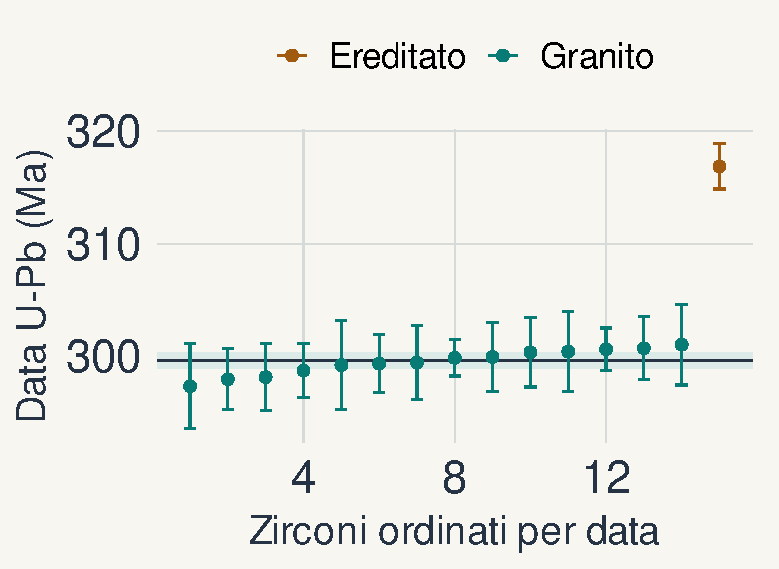
\includegraphics[width=\linewidth,height=6.15cm,keepaspectratio]{Figure/F05.pdf}\par}
\PSmall{Date U-Pb dei quindici zirconi con barre di due deviazioni standard; linea e fascia: media pesata di quattordici zirconi.}
}};
\node[anchor=north west,inner sep=0] at([xshift=10.85cm,yshift=-2.12cm]current page.north west){\Colonna{8.16cm}{\PBody{Quattordici zirconi hanno date fra 297,4 e 301,1 milioni di anni, con incertezze fra 0,8 e 2 milioni di anni. Lo zircone Z15 ha una data di 316,9 milioni di anni, lontana dalle altre di molte deviazioni standard. Uno zircone ereditato è un cristallo più antico che il magma ha incorporato da rocce preesistenti.}
\PSmall{Nel generatore Z15 è un granulo ereditato con età di 318 milioni di anni.}
}};
\end{tikzpicture}\end{frame}

\begin{frame}[plain]\hypertarget{slide26}{}
\bookmark[level=1,page=26]{La media pesata deve includere Z15?}
\begin{tikzpicture}[remember picture,overlay]
\PilotChrome{La media pesata deve includere Z15?}{INCERTEZZA E CONFRONTO DELLE ETÀ}{26}{Un dato si esclude per una ragione documentata: la MSWD segnala il problema, la geologia lo spiega.}
\node[anchor=north west,inner sep=0] at([xshift=.96cm,yshift=-2.12cm]current page.north west){\Colonna{9.40cm}{\PLabel{Domanda}
\PBody{Con tutti i quindici zirconi, la media pesata è coerente con le incertezze? Che cosa cambia escludendo Z15?}
\vspace{.35cm}\PLabel{Interpretazione}
\PBody{Con quindici zirconi la media è $301{,}59\pm0{,}34$ milioni di anni e la MSWD 19,4, oltre la soglia di 1,76. Senza Z15 la media è $299{,}65\pm0{,}36$ e la MSWD 0,58: le date restanti sono coerenti.}
}};
\node[anchor=north west,inner sep=0] at([xshift=10.85cm,yshift=-2.12cm]current page.north west){\Colonna{8.16cm}{\begin{tcolorbox}[enhanced,arc=1.7mm,boxrule=.6pt,colback=white,colframe=Classical!60!Navy,colbacktitle=Navy,coltitle=white,fonttitle=\bfseries\small,title={R · calcolo riproducibile},left=1.7mm,right=1.3mm,top=1.1mm,bottom=1.1mm,before skip=1mm,after skip=1.0mm]\lstinputlisting[style=GeoR,language=R]{Codice/capitolo-08.R}\end{tcolorbox}
\PLabel{Risultato in R}
\begin{tcolorbox}[colback=GeoTint,colframe=Rule,boxrule=.5pt,arc=1.4mm,left=2mm,right=1mm,top=1mm,bottom=1mm]{\fontsize{8.6}{11.4}\selectfont\ttfamily \mbox{\ \ \ \ \ \ \ \ \ \ \ \ media\ \ \ \ se\ \ \ mswd}\\\mbox{tutti\ \ \ \ \ 301.593\ 0.336\ 19.384}\\\mbox{senza\_Z15\ 299.646\ 0.357\ \ 0.583}}\end{tcolorbox}}};
\end{tikzpicture}\end{frame}

\begin{frame}[plain]\hypertarget{slide27}{}
\bookmark[level=1,page=27]{Quando escludere un dato}
\begin{tikzpicture}[remember picture,overlay]
\PilotChrome{Quando escludere un dato}{INCERTEZZA E CONFRONTO DELLE ETÀ}{27}{La ragione per escludere un dato precede il calcolo; la MSWD da sola non basta.}
\node[anchor=north west,inner sep=0] at([xshift=.96cm,yshift=-2.12cm]current page.north west){\Colonna{9.40cm}{\PLabel{Ragioni geologiche}
\PBody{Uno zircone può essere più antico del magma, se ereditato, o più giovane, se ha perso piombo. Le immagini dei cristalli, la posizione dell’analisi e la composizione chimica documentano queste situazioni. Z15 è un caso netto: la sua data dista dalla media di oltre 17 milioni di anni, più di dieci volte la sua incertezza.}
}};
\node[anchor=north west,inner sep=0] at([xshift=10.85cm,yshift=-2.12cm]current page.north west){\Colonna{8.16cm}{\PLabel{Il rischio della selezione}
\PBody{Escludere le date che allontanano la MSWD da 1 finché il valore rientra sotto la soglia produce medie troppo precise. I criteri di esclusione vanno dichiarati prima del calcolo e applicati a tutti i cristalli, e la relazione riporta anche le date escluse.}
\par\smallskip{\centering\adjustbox{max width=.98\linewidth}{$\displaystyle \mathrm{MSWD}=\frac{1}{n-1}\sum_{i=1}^n\frac{(t_i-\bar t)^2}{\sigma_i^2}$}\par\smallskip}
}};
\end{tikzpicture}\end{frame}

\begin{frame}[plain]\hypertarget{slide28}{}
\bookmark[level=1,page=28]{Rb-Sr e U-Pb a confronto}
\begin{tikzpicture}[remember picture,overlay]
\PilotChrome{Rb-Sr e U-Pb a confronto}{INCERTEZZA E CONFRONTO DELLE ETÀ}{28}{Due età si confrontano con la differenza divisa per la sua incertezza combinata.}
\node[anchor=north west,inner sep=0] at([xshift=.96cm,yshift=-2.12cm]current page.north west){\Colonna{9.40cm}{{\centering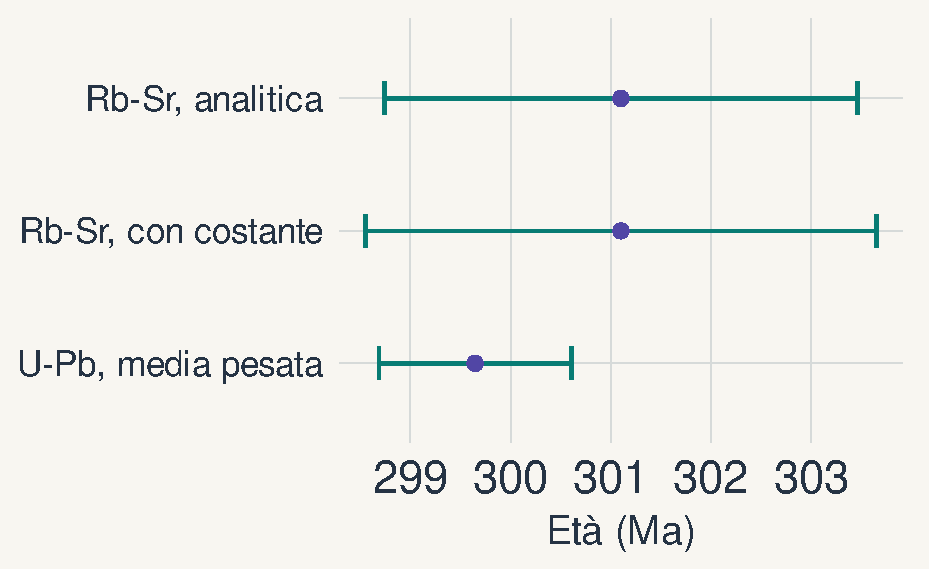
\includegraphics[width=\linewidth,height=6.15cm,keepaspectratio]{Figure/F06.pdf}\par}
\PSmall{Età del granito con barre di due deviazioni standard: isocrona Rb-Sr senza e con la costante di decadimento, media U-Pb.}
}};
\node[anchor=north west,inner sep=0] at([xshift=10.85cm,yshift=-2.12cm]current page.north west){\Colonna{8.16cm}{\PBody{L’isocrona dà $301{,}1\pm1{,}3$ milioni di anni con la costante di decadimento, gli zirconi $299{,}65\pm0{,}48$ includendo l’incertezza della costante di ${}^{238}$U. La differenza, 1,46 milioni di anni, vale 1,07 volte la sua incertezza combinata: le due età sono compatibili.}
\par\smallskip{\centering\adjustbox{max width=.98\linewidth}{$\displaystyle z=\frac{t_1-t_2}{\sqrt{\sigma_1^2+\sigma_2^2}}$}\par\smallskip}
}};
\end{tikzpicture}\end{frame}

\begin{frame}[plain]\hypertarget{slide29}{}
\bookmark[level=1,page=29]{Media pesata e dispersione geologica}
\begin{tikzpicture}[remember picture,overlay]
\PilotChrome{Media pesata e dispersione geologica}{INCERTEZZA E CONFRONTO DELLE ETÀ}{29}{Valutare la media pesata quando le date hanno una dispersione reale oltre a quella analitica.}
\node[anchor=north west,inner sep=0] at([xshift=.96cm,yshift=-2.12cm]current page.north west){\Colonna{9.40cm}{{\centering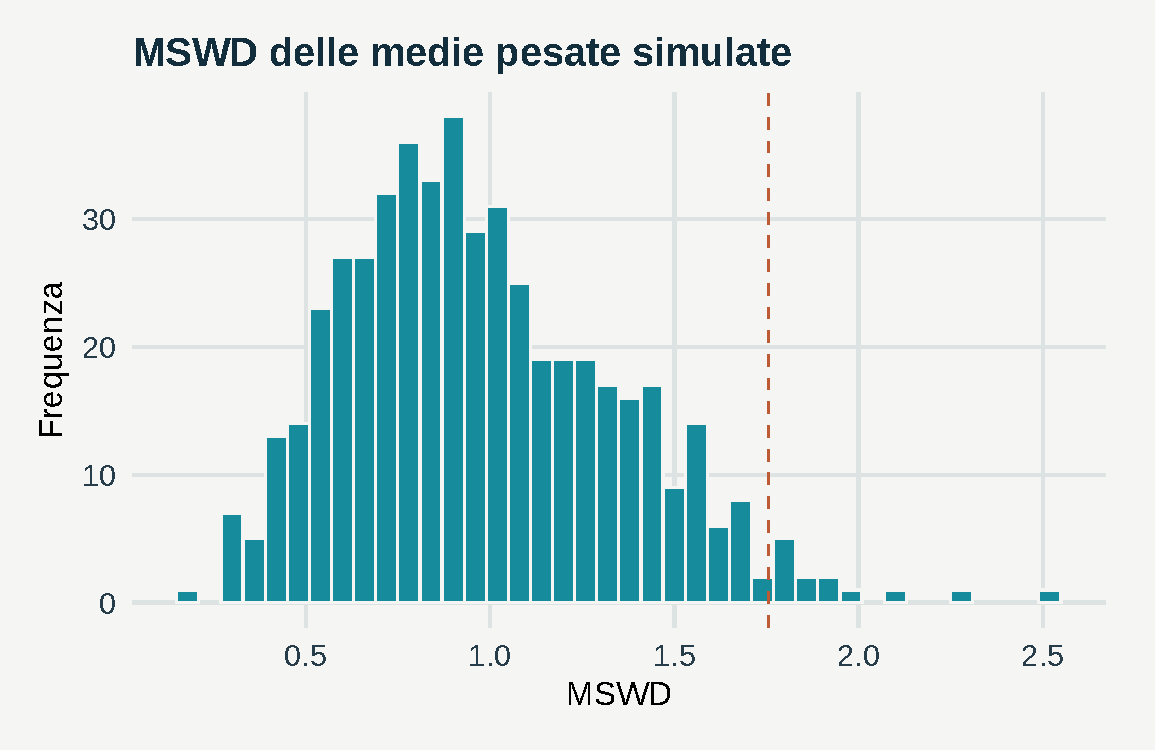
\includegraphics[width=\linewidth,height=6.0cm,keepaspectratio]{Esperimenti/m19-media-A.pdf}\par}
\PSmall{Dispersione geologica: 0 Ma; quindici cristalli; cinquecento gruppi. Seme: 17.}
}};
\node[anchor=north west,inner sep=0] at([xshift=10.85cm,yshift=-2.12cm]current page.north west){\Colonna{8.16cm}{\PLabel{Scenario A · simulazione}
\PBody{L’esperimento simula cinquecento gruppi di date attorno a 300 milioni di anni, con incertezze analitiche fra 0,8 e 2 e una dispersione geologica impostata. Senza dispersione la MSWD media è 0,97 e l’intervallo nominale contiene 300 nel 95,6\% dei gruppi.}
\par\smallskip{\centering\adjustbox{max width=.98\linewidth}{$\displaystyle \bar t=\frac{\sum_i t_i/\sigma_i^2}{\sum_i 1/\sigma_i^2}$}\par\smallskip}
\PSmall{L’errore scalato moltiplica l’errore standard per $\sqrt{\mathrm{MSWD}}$ quando la MSWD supera 1.}
}};
\node[anchor=north east,inner sep=0] at([xshift=17.1cm,yshift=-12.04cm]current page.north west){\fontsize{7.7}{9}\selectfont \href{https://marzione00.github.io/Lab_Geo/\#laboratorio/m19-media}{\color{Classical}\bfseries Apri il laboratorio · m19-media}};
\end{tikzpicture}\end{frame}

\begin{frame}[plain]\hypertarget{slide30}{}
\bookmark[level=1,page=30]{Confronto | Media pesata e dispersione geologica}
\begin{tikzpicture}[remember picture,overlay]
\PilotChrome{Confronto | Media pesata e dispersione geologica}{INCERTEZZA E CONFRONTO DELLE ETÀ}{30}{Con dispersione geologica l’errore nominale della media pesata è troppo piccolo.}
\node[anchor=north west,inner sep=0] at([xshift=.96cm,yshift=-2.12cm]current page.north west){\Colonna{9.40cm}{{\centering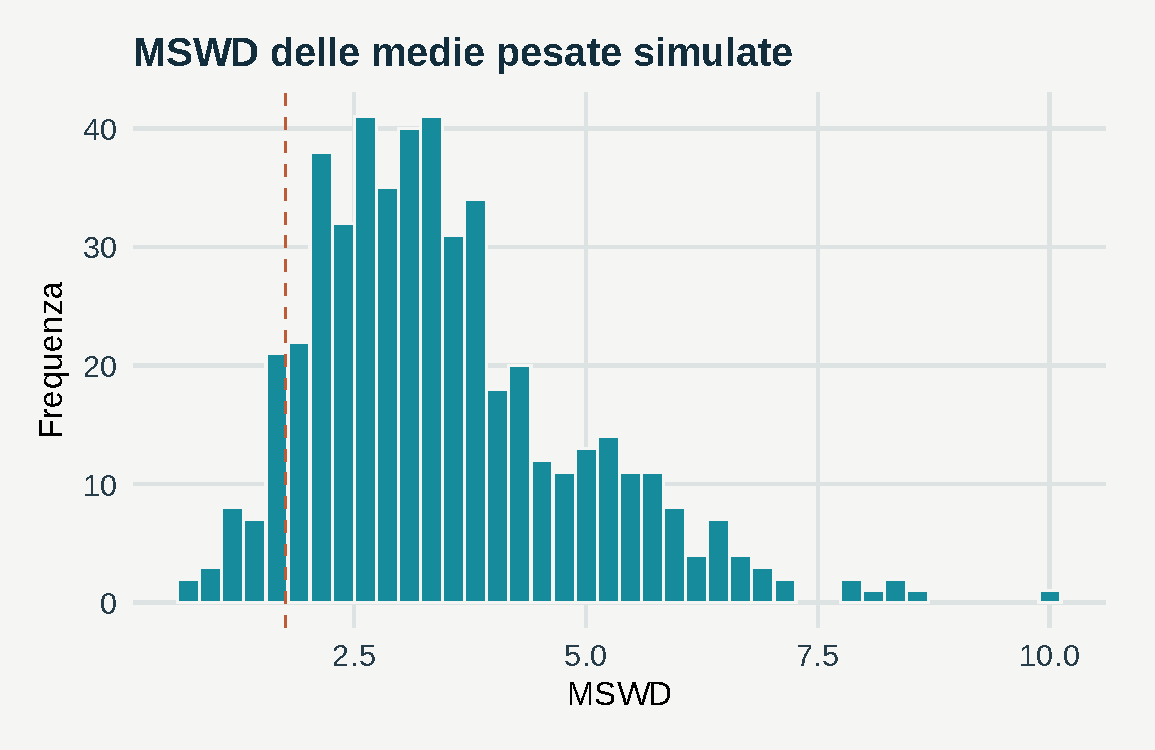
\includegraphics[width=\linewidth,height=5.6cm,keepaspectratio]{Esperimenti/m19-media-B.pdf}\par}
\PSmall{Dispersione geologica: 0 $\to$ 2 Ma. Tutti gli altri parametri e il seme sono fissi.}
}};
\node[anchor=north west,inner sep=0] at([xshift=10.85cm,yshift=-2.12cm]current page.north west){\Colonna{8.16cm}{\PLabel{Confronto fra gli scenari}
{\fontsize{10.2}{12.8}\selectfont\begin{tabular}{@{}>{\raggedright\arraybackslash}p{0.48\linewidth}@{\hspace{.13cm}}>{\raggedright\arraybackslash}p{0.224\linewidth}@{\hspace{.13cm}}>{\raggedright\arraybackslash}p{0.224\linewidth}@{}}\toprule Grandezza & A & B\\[2.3pt]
\midrule 
MSWD medio & 0{,}974 & 3{,}46\\[2.3pt]
Quota oltre la soglia & 0{,}026 & 0{,}924\\[2.3pt]
Copertura, errore nominale & 0{,}956 & 0{,}65\\[2.3pt]
Copertura, errore scalato & 0{,}962 & 0{,}886\\[2.3pt]
\bottomrule\end{tabular}\par}
\vspace{.25cm}\PBody{Con 2 milioni di anni di dispersione la MSWD media sale a 3,46 e la copertura nominale scende al 65\%; l’errore scalato la riporta all’88,6\%, ancora sotto il 95\%.}
}};
\node[anchor=north east,inner sep=0] at([xshift=17.1cm,yshift=-12.04cm]current page.north west){\fontsize{7.7}{9}\selectfont \href{https://marzione00.github.io/Lab_Geo/\#laboratorio/m19-media}{\color{Classical}\bfseries Apri il laboratorio · m19-media}};
\end{tikzpicture}\end{frame}

\begin{frame}[plain]\hypertarget{slide31}{}
\bookmark[level=0,page=31]{Sintesi}
\bookmark[level=1,page=31]{Dal risultato alla relazione}
\begin{tikzpicture}[remember picture,overlay]
\PilotChrome{Dal risultato alla relazione}{SINTESI}{31}{Riporta età, incertezza, MSWD, numero di campioni, costante di decadimento e criteri di esclusione.}
\node[anchor=north west,inner sep=0] at([xshift=.96cm,yshift=-2.12cm]current page.north west){\Colonna{9.40cm}{\PLabel{Domanda di partenza}
\PBody{Quanti anni ha il granito, e con quale incertezza?}
\PLabel{Risultato da discutere}
\PBody{L’isocrona Rb-Sr del granito dà $301{,}1\pm1{,}2$ milioni di anni con MSWD 0,50 e rapporto iniziale 0,708506; con la costante di decadimento l’incertezza è 1,3. Gli zirconi, escluso il granulo ereditato, danno $299{,}65\pm0{,}36$. Il filone ha una dispersione in eccesso e un’età di $247{,}5\pm2{,}4$ con l’incertezza scalata.}
}};
\node[anchor=north west,inner sep=0] at([xshift=10.85cm,yshift=-2.12cm]current page.north west){\Colonna{8.16cm}{\PLabel{Limiti della conclusione}
\PBody{I dati sono sintetici e gli errori dei due rapporti sono indipendenti. Le incertezze sono a una deviazione standard; la scalatura per la MSWD presuppone un eccesso proporzionale agli errori analitici, e l’esclusione di Z15 si basa sul modello che ha generato i dati.}
\vspace{.4cm}\href{https://marzione00.github.io/Lab_Geo/\#modulo-M19}{\color{Classical}\bfseries Torna agli esperimenti di Isocrona}
}};
\end{tikzpicture}\end{frame}

\begin{frame}[plain]\hypertarget{slide32}{}
\bookmark[level=0,page=32]{Riferimenti}
\bookmark[level=1,page=32]{Fonti, dati e codice per riprodurre le figure}
\begin{tikzpicture}[remember picture,overlay]
\PilotChrome{Fonti, dati e codice per riprodurre le figure}{RIFERIMENTI}{32}{I risultati numerici si riferiscono ai dati e alle ipotesi dichiarate nel caso.}
\node[anchor=north west,inner sep=0] at([xshift=.96cm,yshift=-2.12cm]current page.north west){\Colonna{9.40cm}{\PLabel{Fonti}
{\fontsize{9.4}{12.2}\selectfont G. A. McIntyre e colleghi, Journal of Geophysical Research 71(22), 5459, 1966.\par I. Wendt e C. Carl, Chemical Geology 86(4), 275–285, 1991.\par A. P. Dickin, Radiogenic Isotope Geology, Cambridge University Press, 1995.\par D. York e colleghi, American Journal of Physics 72(3), 367–375, 2004.\par I. M. Villa e colleghi, Geochimica et Cosmochimica Acta 164, 382–385, 2015.\par I. M. Villa e colleghi, Pure and Applied Chemistry 94(9), 1085–1092, 2022.\par P. Vermeesch, High MSWDs are not the problem, low ones are, 2025.\par}
}};
\node[anchor=north west,inner sep=0] at([xshift=10.85cm,yshift=-2.12cm]current page.north west){\Colonna{8.16cm}{\PLabel{Dati e codice}
\PBody{Dati sintetici del corso (isocrone\_v1.csv, date\_v1.csv), generati da R/genera\_dati.R. R/york.R contiene la regressione di York; Codice contiene i frammenti delle pagine; R/M19\_figure.R ricostruisce figure e valori; Esperimenti contiene i programmi dei due scenari e Diagrammi i disegni TikZ.}
\vspace{.3cm}\href{https://marzione00.github.io/Lab_Geo/\#lezione-M19}{\color{Classical}\bfseries Apri le tappe di Isocrona su GeoStat Lab}
}};
\end{tikzpicture}\end{frame}
\end{document}
